\documentclass[a4paper, 12pt]{article}
\usepackage{amsmath, amssymb}
\usepackage{geometry}  % 控制页面边距
\usepackage{graphicx}  % 插入图片 
\usepackage{float}     % 强制图片在当前位置
\usepackage{hyperref}  % 目录可以跳转
\usepackage{xcolor}    % 字体颜色
    % Define a custom light blue color
    \definecolor{light-blue}{RGB}{0, 129, 255} % Light blue (using RGB values)
\geometry{left=2.5cm, right=2.5cm, top=2.5cm, bottom=2.5cm}

\usepackage{fancyhdr}  % 页眉和页脚
\pagestyle{fancy}
\fancyhf{}  % 清除默认设置
\fancyhead[L]{Database Review Notes}  % 左侧页眉内容
\fancyhead[R]{}  % 确保右侧页眉清除
\fancyfoot[C]{\thepage}  % 页脚显示页码

\setlength{\parindent}{0pt} % 取消缩进

% 标题与图片
\title{
    
\includegraphics[width=0.8\textwidth]{Yanami_ep1.JPG}\\  % 确保图片路径正确
    Database REVIEW
}
\author{Kinoko}
\date{\today}

\begin{document}

\pagenumbering{gobble}  % 禁用页码

\begin{titlepage}  
    \maketitle
\end{titlepage}

\pagenumbering{roman}  % 使用罗马数字
\fancyhead[R]{}  % 禁用右侧页眉

% 插入目录页
\tableofcontents
\newpage  % 目录单独一页

\pagenumbering{arabic}  % 设置为阿拉伯数字

\section*{Course Syllabus}  % 无编号的章节
\fancyhead[R]{September 23, 2024}  % 手动设置日期
\addcontentsline{toc}{section}{Course Syllabus}  % 手动添加到目录中
    \begin{center}
        \begin{enumerate}
        \renewcommand{\labelenumi}{\Roman{enumi}.}  % 将编号改为大写罗马数字
        \item General Introduction
        \item Relational Model
        \item SQL
        \item Database Security
        \item Database Integrity
        \item Relational Database Theory 
        \item Relational Database Design
        \item Query Processing and Optimization
        \item Database Recovery
        \item Concurrency Control
    \end{enumerate}
    \end{center}
    

\newpage

% 设置章节从 1 开始编号
\setcounter{section}{0}

\section{1A: General Introduction}
\fancyhead[R]{September 23, 2024}  % 手动设置日期
    \subsection{What is data?}
        \begin{itemize}
            \item Data is just the data and information that can be stored.
            \item it is typically \textbf{unprocessed} and \textbf{raw}.
            \item Once we have put our data into \textbf{context}, \textbf{data is transformed into information}, which
            is then used to make decisions.
        \end{itemize}
    
    \subsection{Databases, Data, and Information}
        Database
        \begin{itemize}
            \item Collection of data organized in a manner that allows access, retrieval, and use of
        \end{itemize}

        Data
        \begin{itemize}
            \item Collection of unprocessed items
            \item Text, Numbers, Images, Audio, Video
        \end{itemize}

        Information
        \begin{itemize}
            \item Processed data
            \item organized, meaningful, useful
        \end{itemize}

    \subsection{What is Database?}
    Database = A large collection of related
    data
    \subsection{Database Management System (DBMS)}
    \begin{itemize}
        \item Compilation of related data
        \item A collection of programs for accessing data
        \item A database management system (DBMS) stores information about a specific
        organization.
        \item Reliable and easy to use
    \end{itemize}

    \subsection{DBMS Core Functions}
    DBMS gives us an interface or tool to carry out a variety of tasks, including building databases,
    storing data in them, updating data, creating tables in the databases, and much more.
    \begin{itemize}
        \item Defining a particular database in terms of\\
        \textbf{its data types ,structures , and constraints} 
        \item Manipulating the database
        \begin{itemize}
            \item Retrieval: Querying, generating reports
            \item Modification: Insertions, deletions and updates to its content
            \item Accessing the database through Web applications
        \end{itemize}
        \item Processing and sharing by a set of concurrent users and application programs
        yet, keeping all data valid and consistent.
    \end{itemize}

    \subsection{DBMS Con.}
    Additionally, DBMS offers security and protection to the
    databases.\\
    Maintaining data consistency when multiple users are
    present.\\
    Example of DBMS software: MySql, Oracle, Ms SQL Server

    \subsection{Types of Database}
    \begin{itemize}
        \item Traditional Applications:
        \begin{itemize}
            \item Numeric and Textual Databases
        \end{itemize}
        \item More Recent Applications:
        \begin{itemize}
            \item Multimedia Database (images, audio, video…)
            \item Geographic Information Systems (GIS): Store and analyze maps, weather data, and satellite images
        \end{itemize}
        \item Data Warehouses and online analytical processing (OLAP) systems
        \begin{itemize}
            \item Extract and analyze useful business information from very
            large databases.
            \item Support decision making.
        \end{itemize}
        \item Real-time and Active Databases
        \begin{itemize}
            \item A real-time database is a database system that processes
            data in real time to handle workloads that are constantly
            changing.
        \end{itemize}
    \end{itemize}

    \subsection{The Database approach's main characteristics}
    \begin{itemize}
        \item Data Abstraction
            \begin{itemize}
                \item A data model hides storage details while providing users with a conceptual view of the database.
                \item Programs refer to the data model constructs rather than data storage details.
            \end{itemize}
        \item Multiple data views are supported
            \begin{itemize}
                \item Each user may see a different view of the database that only shows the data that is relevant to them.
            \end{itemize}
        \item Data sharing and transaction processing for multiple users
            \begin{itemize}
                \item Allowing multiple users to access and update the database at the same time.
                \item The recovery subsystem ensures that the effect of each completed transaction is permanently recorded in the database.
                \item Database applications rely heavily on OLTP (Online Transaction Processing). 
                Hundreds of concurrent transactions can be executed per second as a result of this.                
            \end{itemize}
    \end{itemize}

\newpage
\section{1B: General Introduction}
\fancyhead[R]{October 10, 2024}
    \subsection{Data models}
    A data model is a set of concepts for display data.\\
    - The most widely used data model is the \textcolor{red}{relational model}.\\
    - \textcolor{red}{Entity relational model}
    \subsection{Data Abstraction in db}
        \begin{itemize}
            \item Abstraction is one of the main features of database systems
            \item Keeping \textcolor{red}{irrelevant information hidden} from users and giving them an
            abstract view of the data makes user-database interaction simple and
            effective
            \item These constraints are hidden from users so that they can simply \textcolor{green}{access
            the data}, and \textcolor{green}{just the relevant portion} of the database is made \textcolor{green}{visible
            to them} through data abstraction.
        \end{itemize}
    \subsection{Level of data abstraction}
    \begin{figure}[H]
        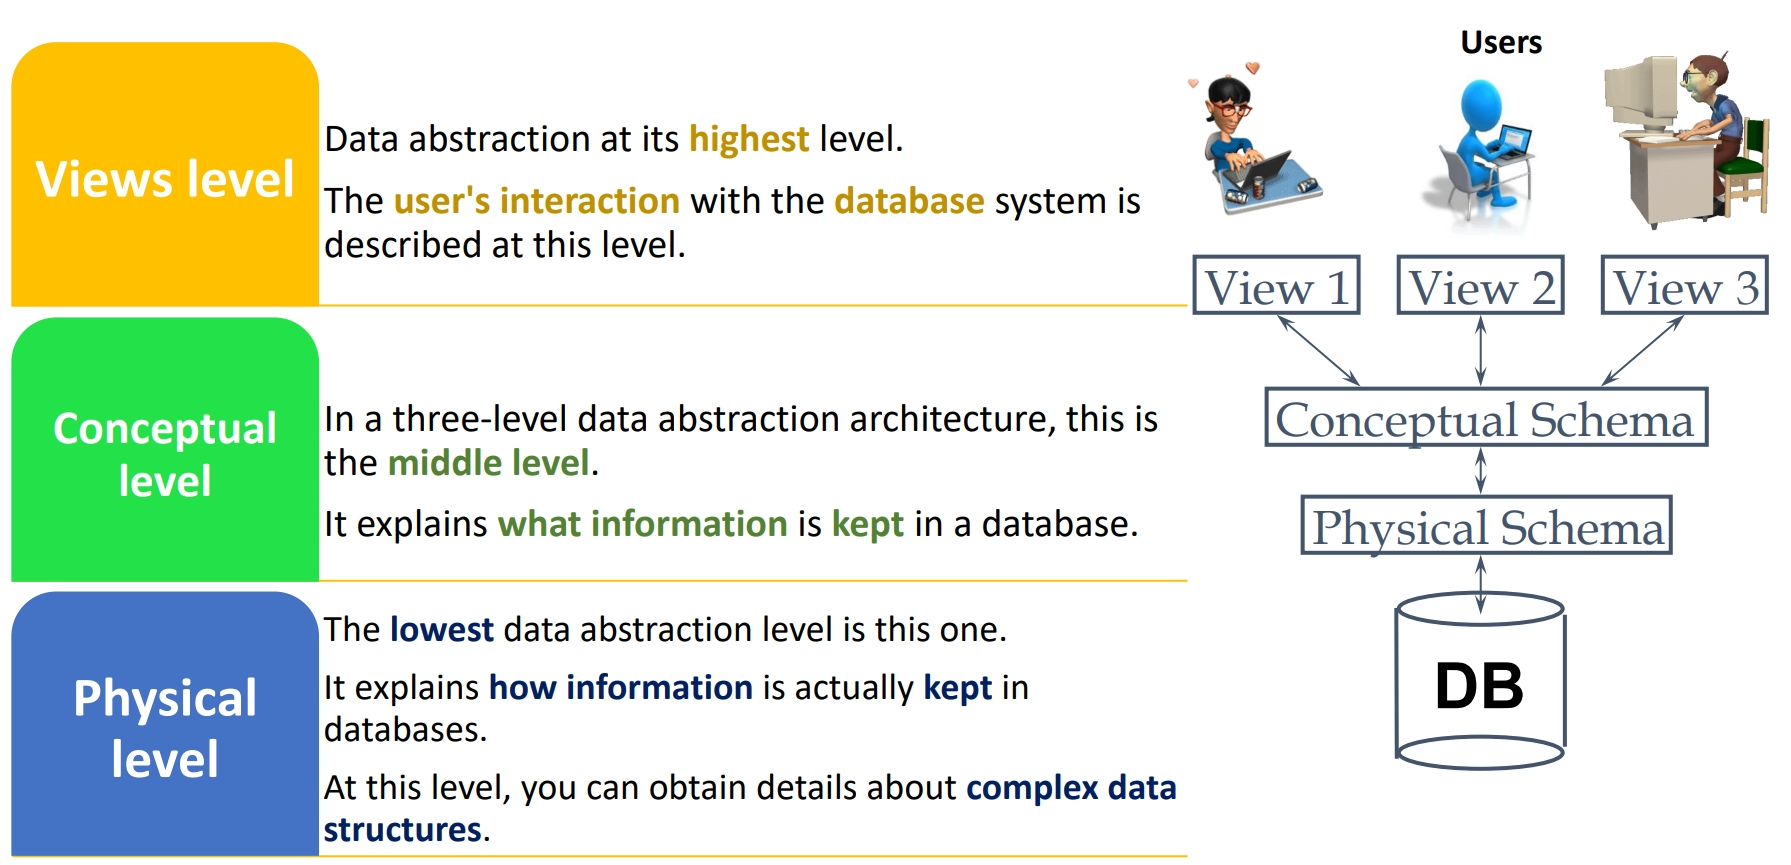
\includegraphics[width=\textwidth]{chapter1a_1.png}
    \end{figure}
    logical level: blueprint of data

\newpage
\section{2A: Relational Model}
\fancyhead[R]{October 10, 2024}
    \subsection{Relational Model Concepts}
    \textcolor{purple}{Represent data as a collection of relations}\\
    - row(tuple)\\
    - column(attribute)
    \begin{figure}[H]
        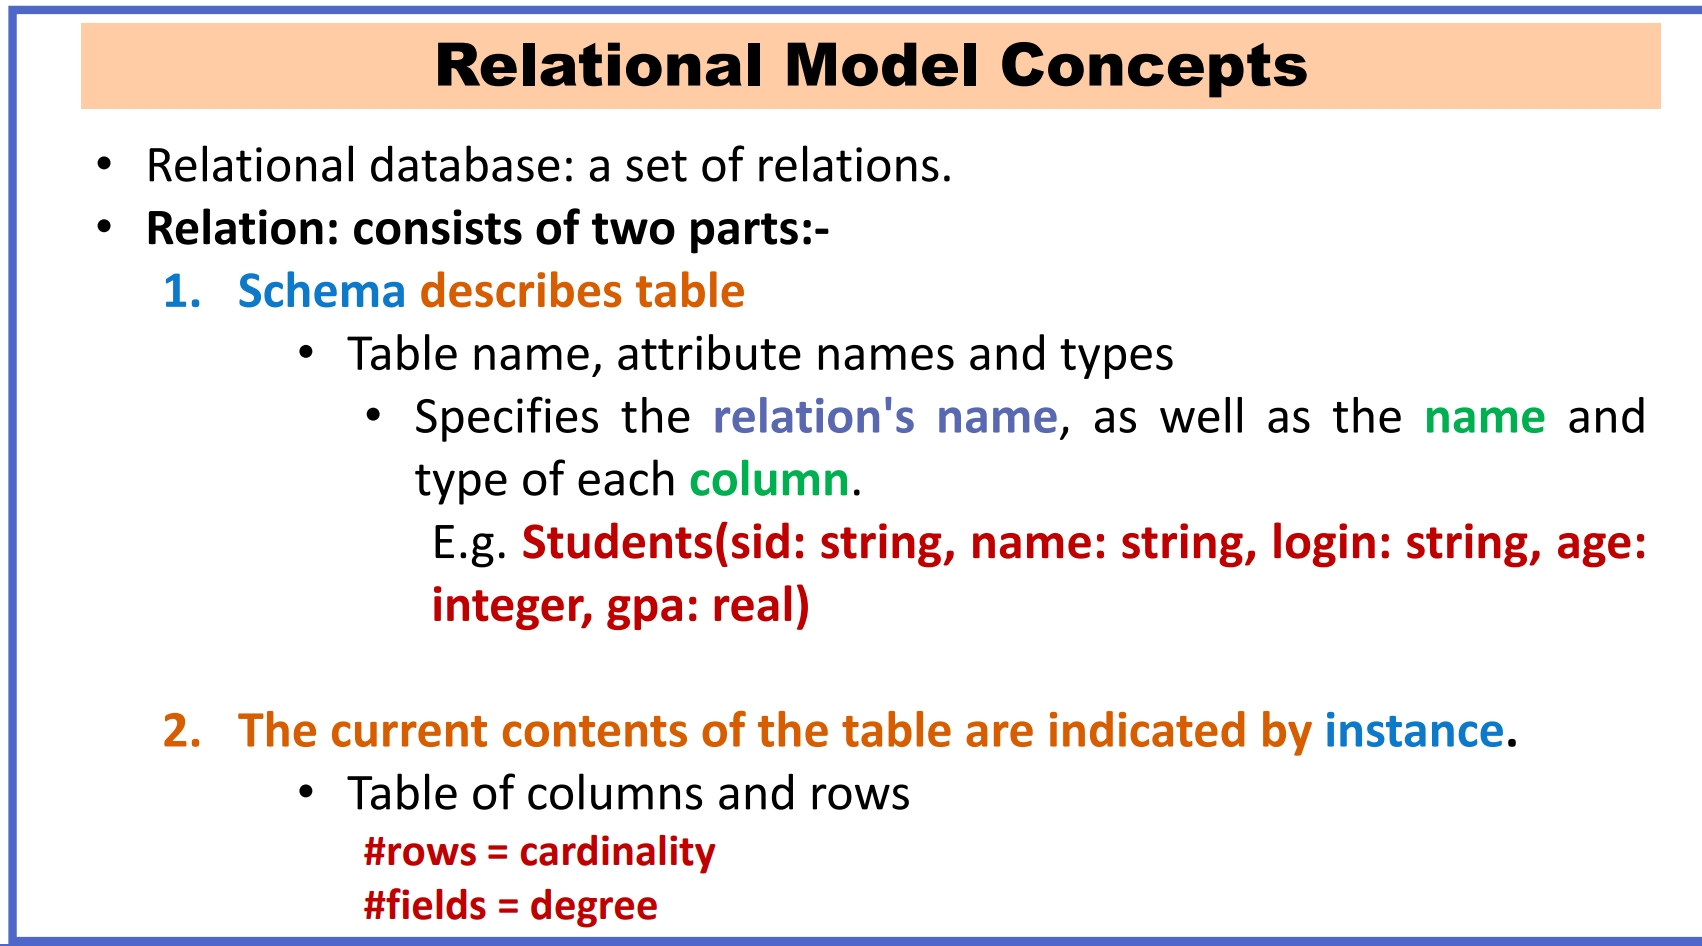
\includegraphics[width=\textwidth]{chapter1a_2.png}
        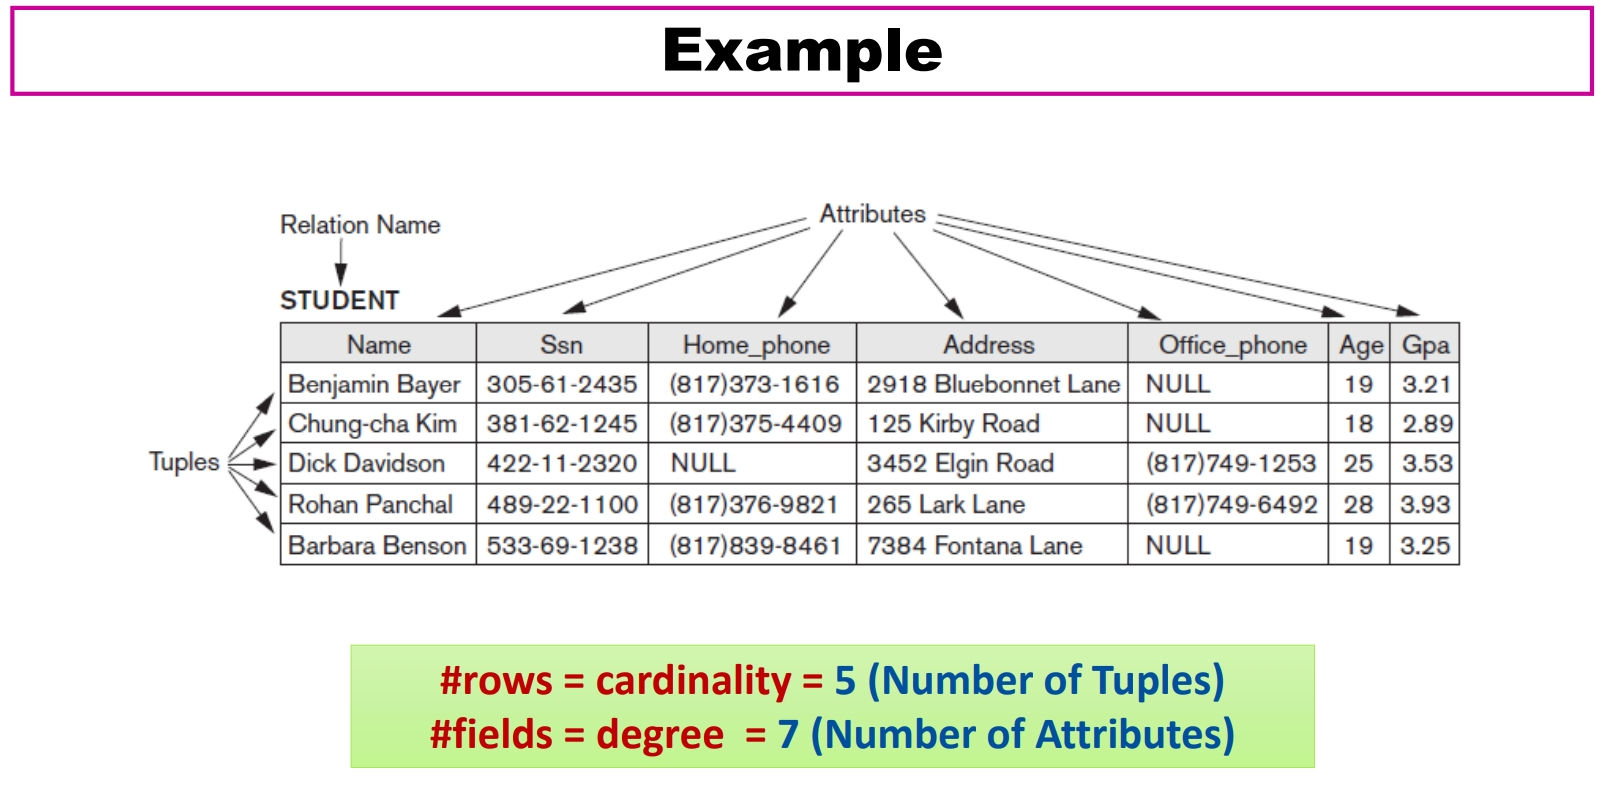
\includegraphics[width=\textwidth]{chapter1a_3.png}
    \end{figure}
    \vspace{3cm}
    \subsection{Basic Structure}
    \subsubsection{Characteristics of Relaions}
        \begin{itemize}
            \item A Relation initially was a mathematical concept based on the ideas of \textcolor{orange}{sets}.
            \item The relation above also have \textcolor{red}{keys}, such as: Primary Key, Foreign Key
        \end{itemize}
    \subsubsection{Constraints}
    \begin{figure}[H]
        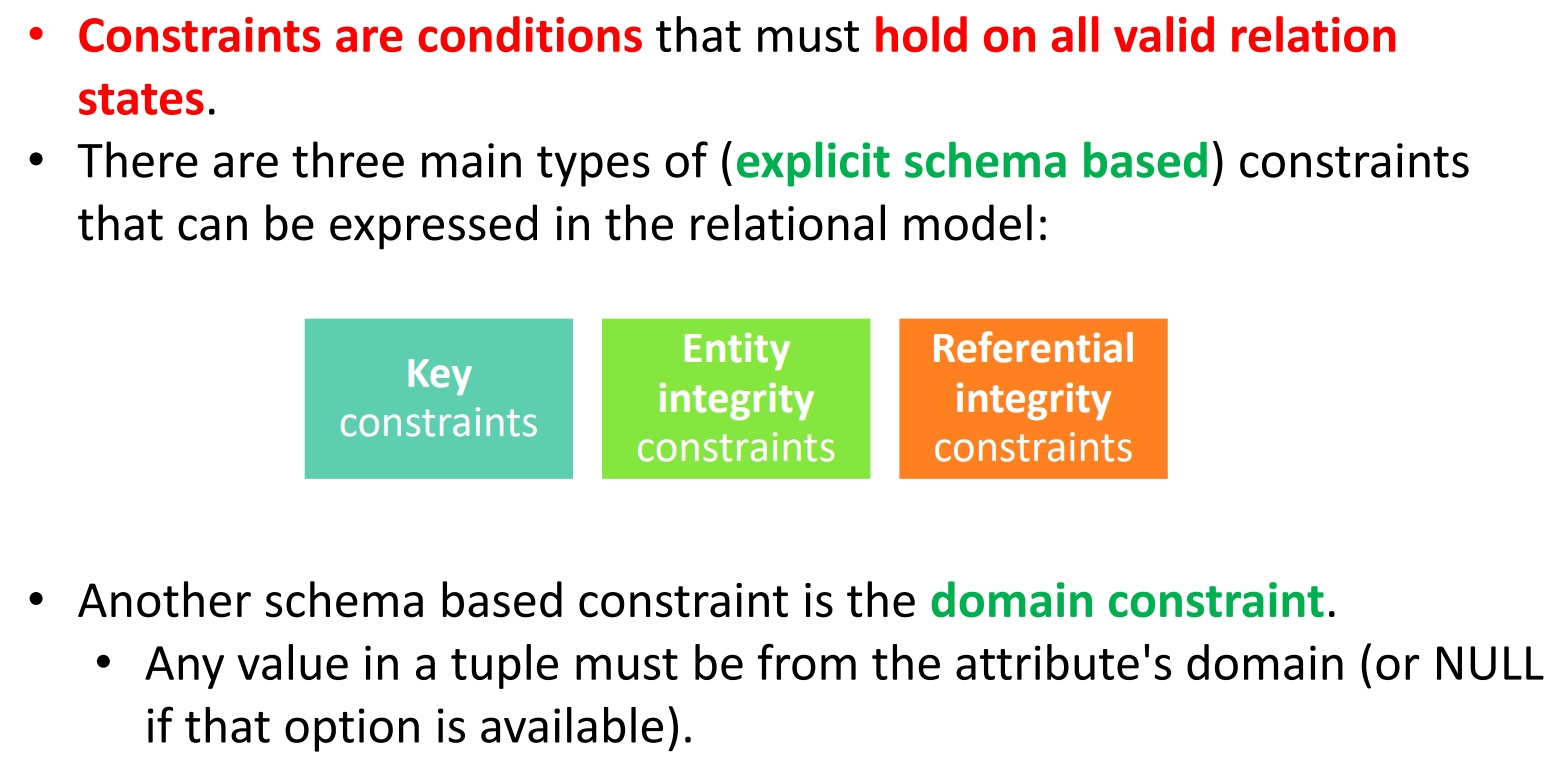
\includegraphics[width=\textwidth]{chapter1a_4.png}
        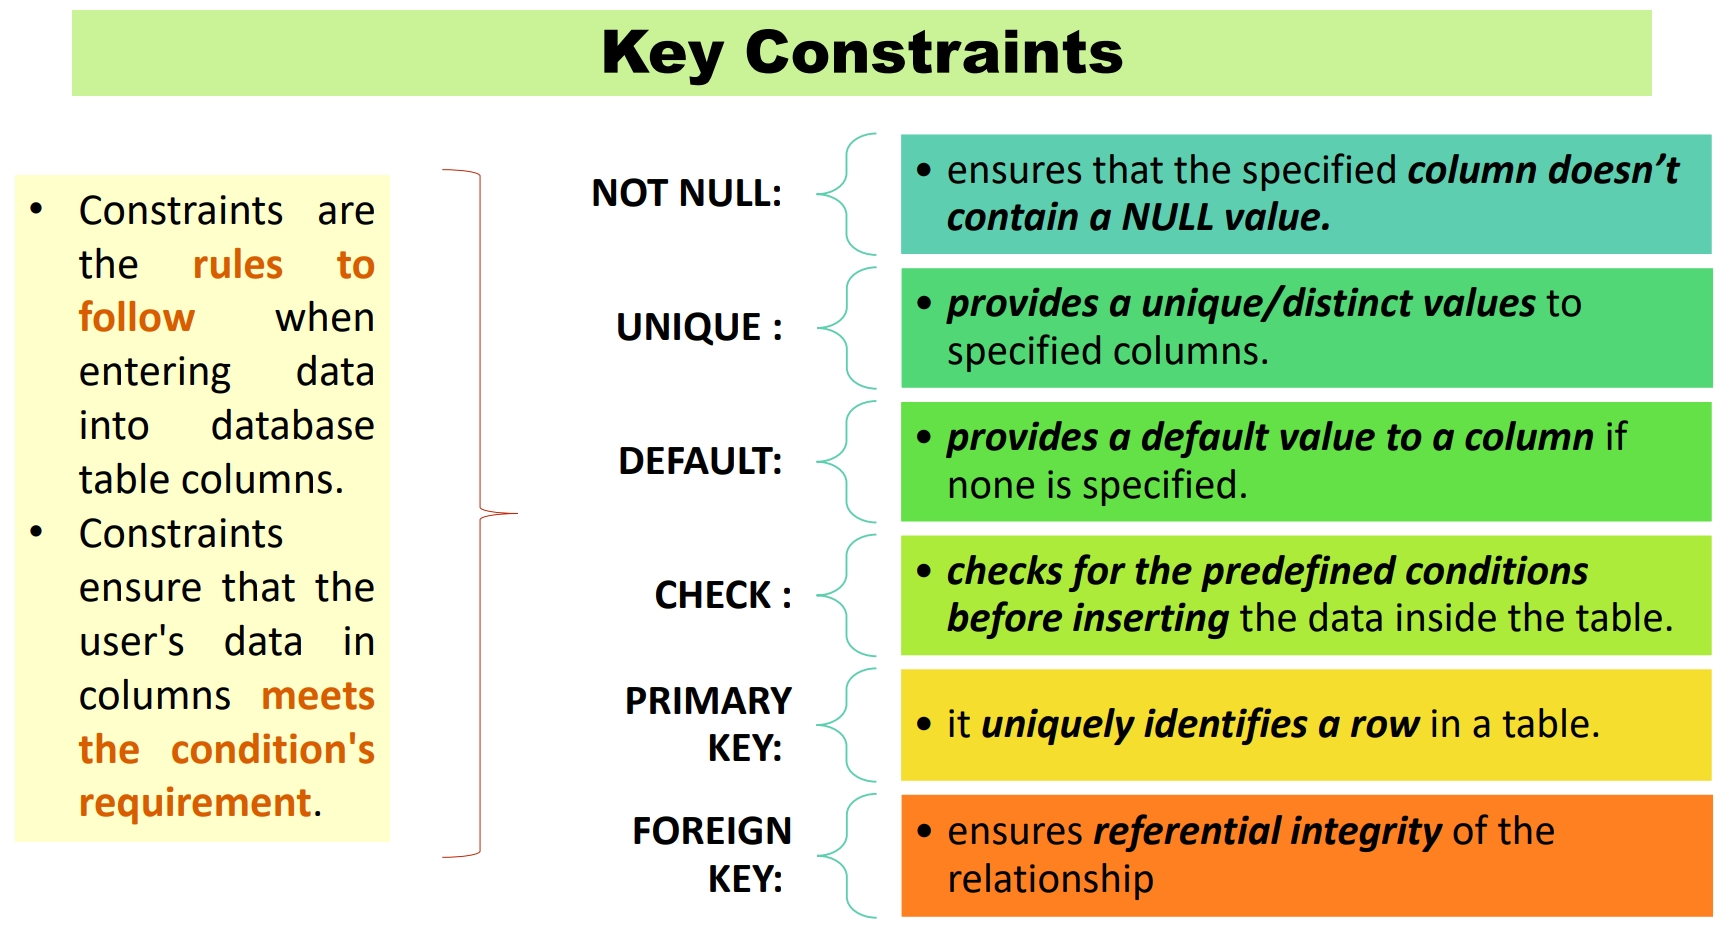
\includegraphics[width=\textwidth]{chapter1a_5.png}
    \end{figure}
    \subsubsection{Relational Database Schema}
    \begin{figure}[H]
        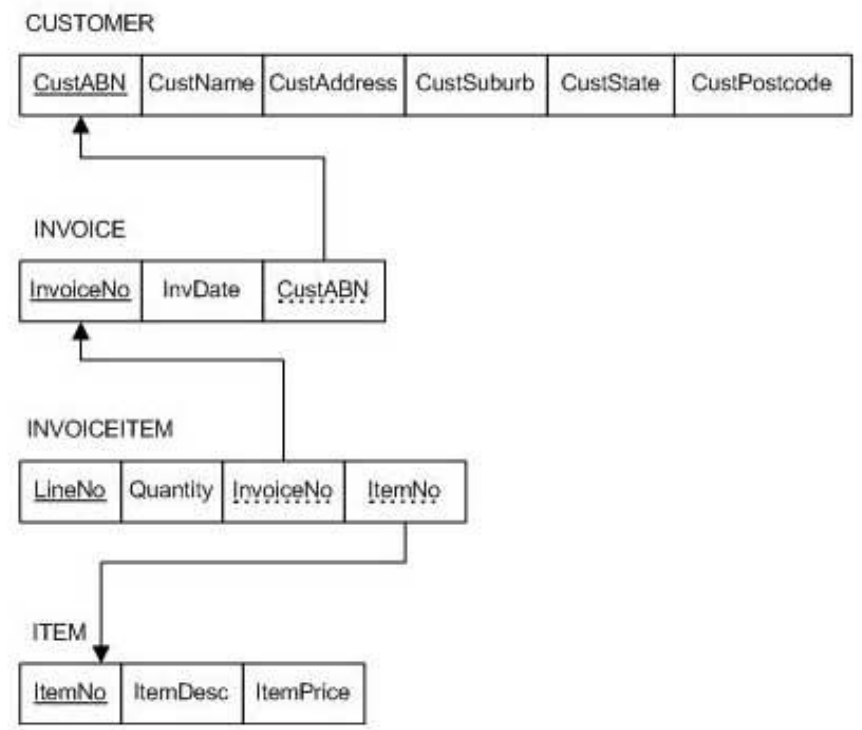
\includegraphics[width=0.4\textwidth]{chapter1a_6.png}
    \end{figure}

    \subsection{Relational Algebra}
    \subsubsection{Query Language}
    A Language which is used to \textcolor{red}{store} and \textcolor{red}{retrieve data} from
    database is known as query language.(e.g. SQL)
    \subsubsection{Relational Algebra in Database}
    \begin{figure}[H]
        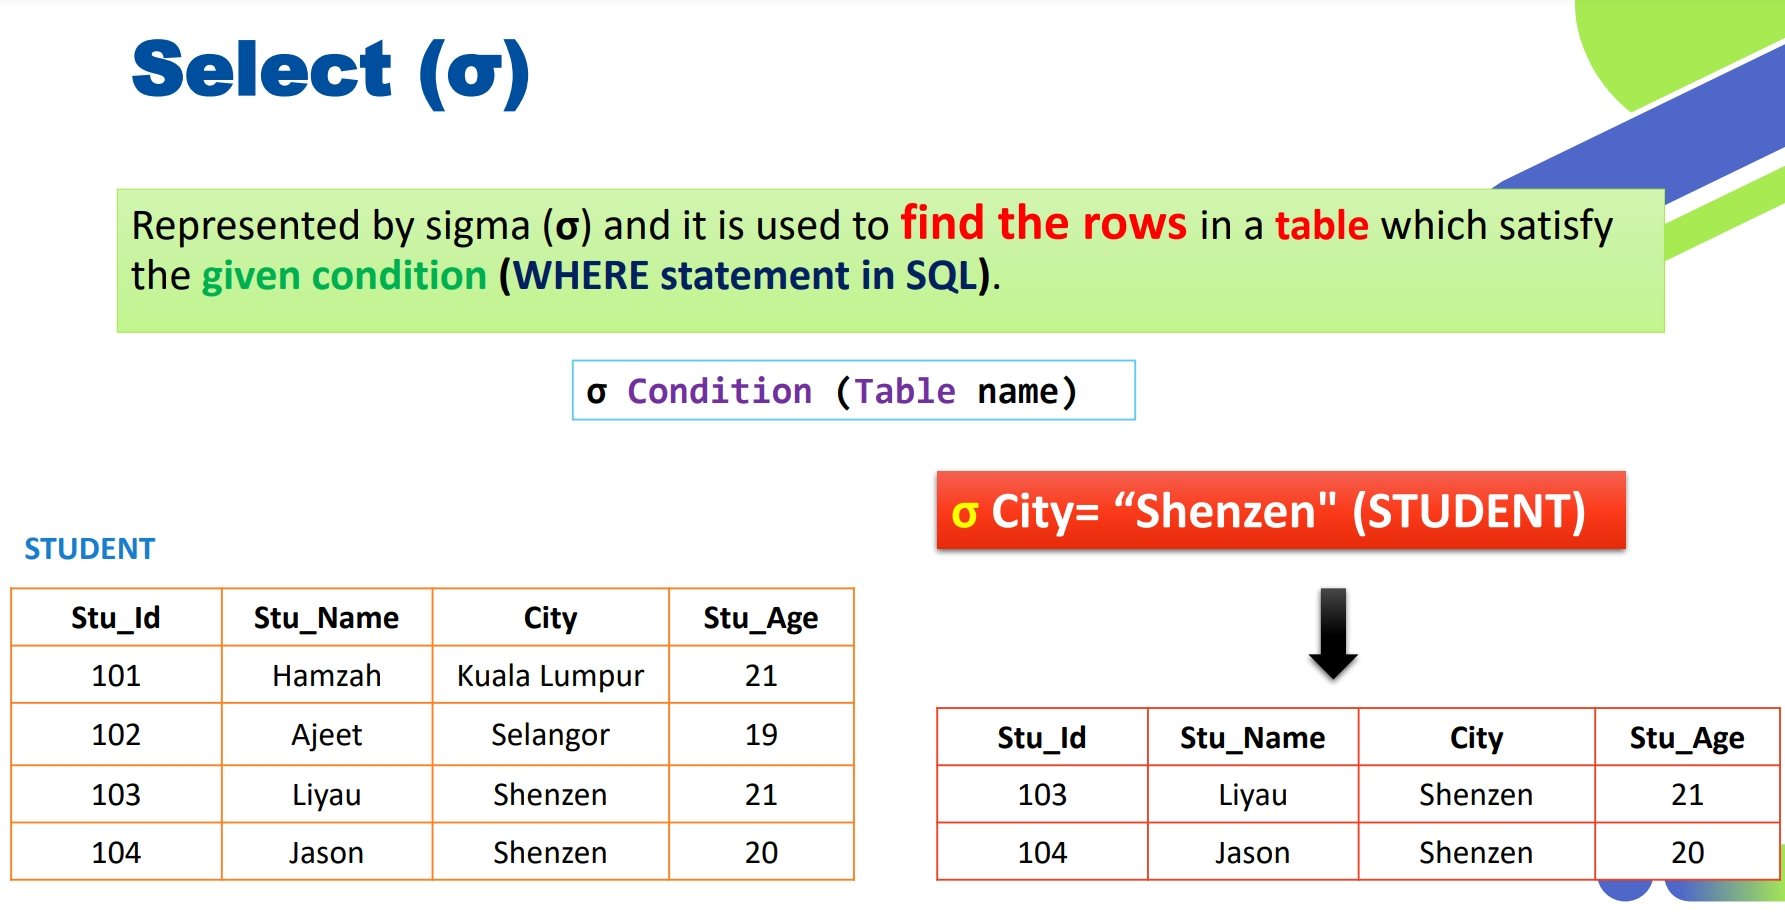
\includegraphics[width=0.8\textwidth]{chapter1a_7.png}
        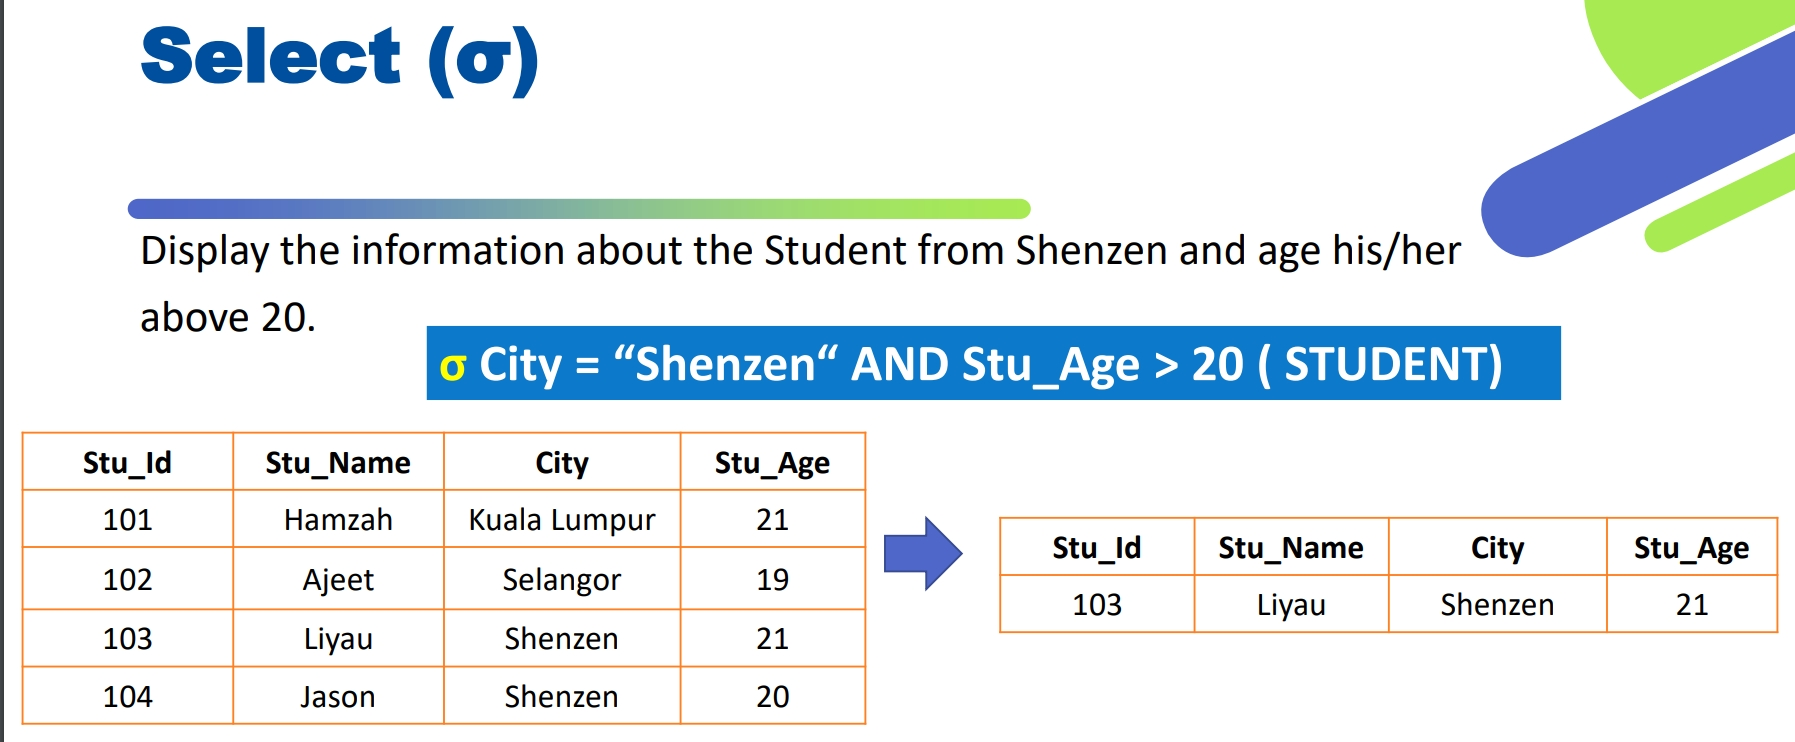
\includegraphics[width=0.8\textwidth]{chapter1a_8.png}
    \end{figure}
    \begin{figure}[H]
        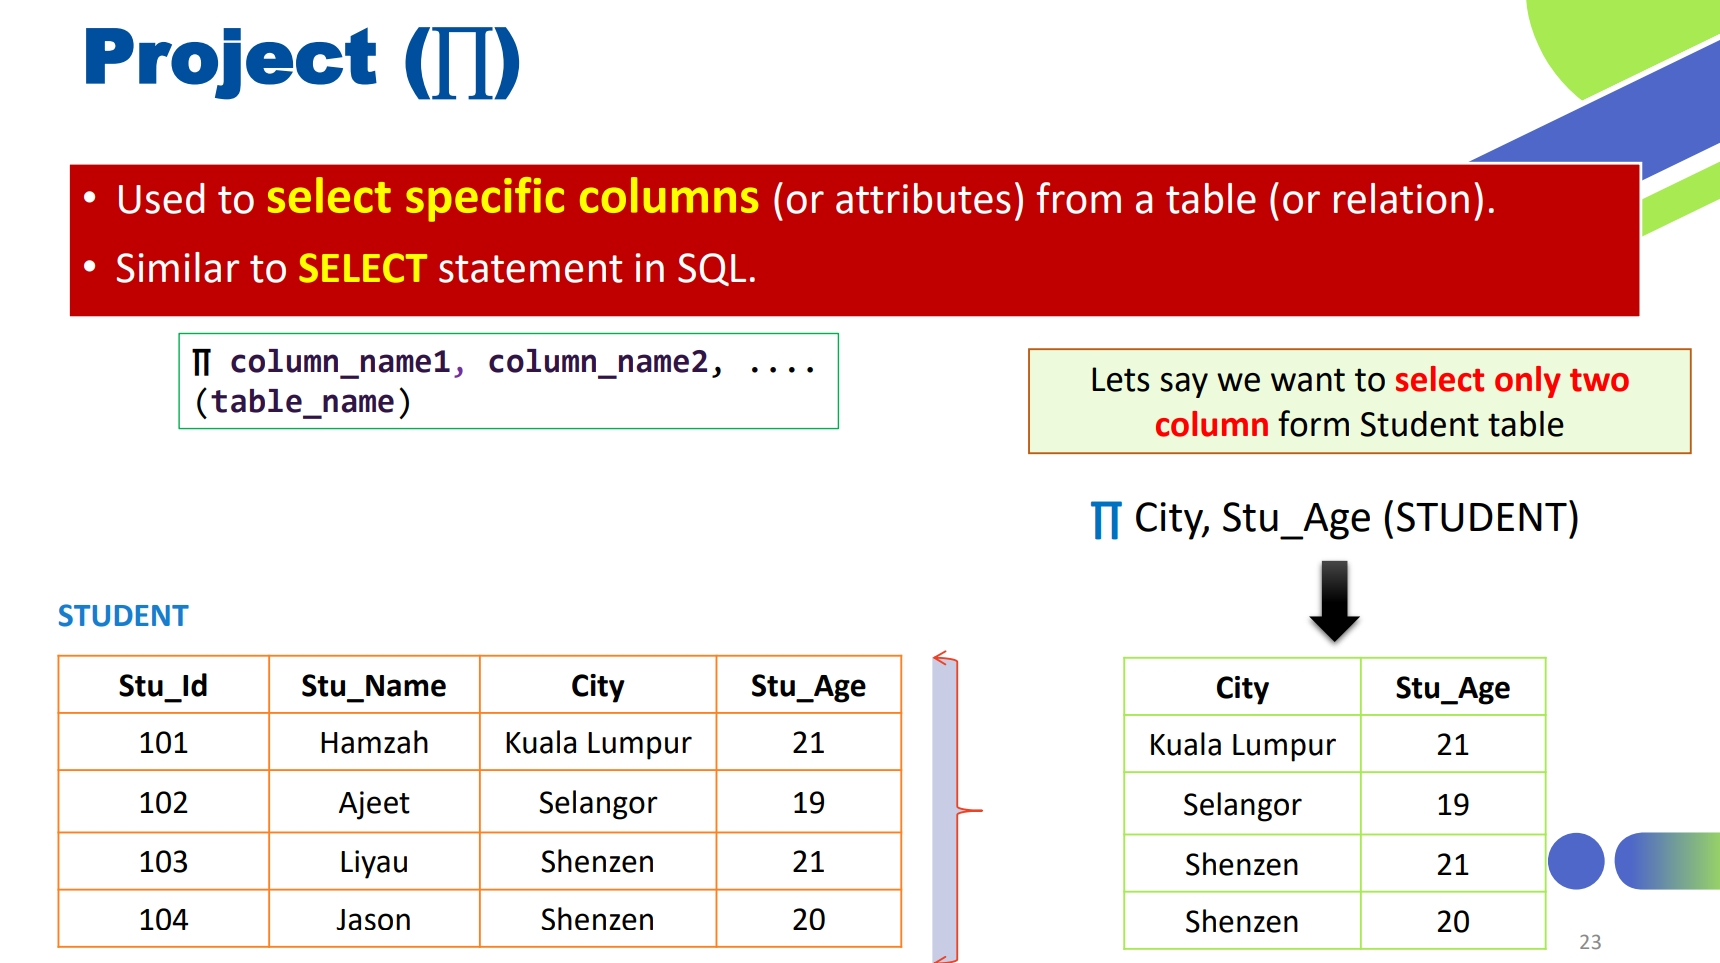
\includegraphics[width=0.9\textwidth]{chapter1a_9.png}
        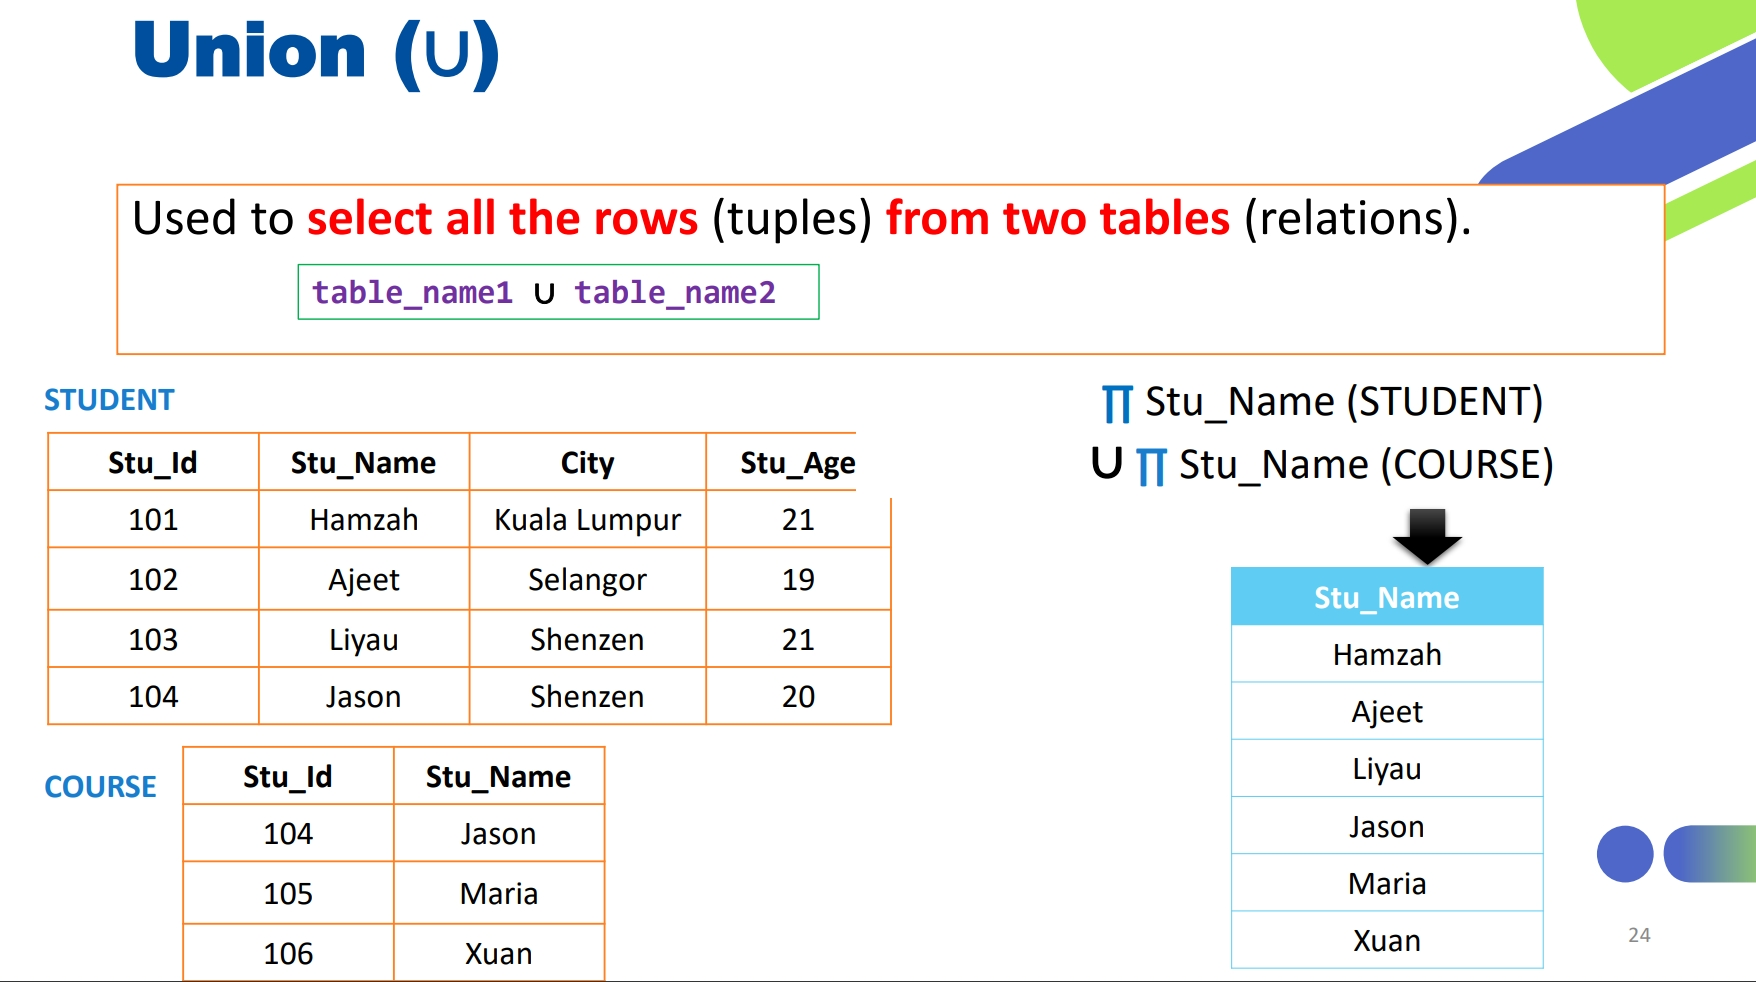
\includegraphics[width=0.9\textwidth]{chapter1a_10.png}
        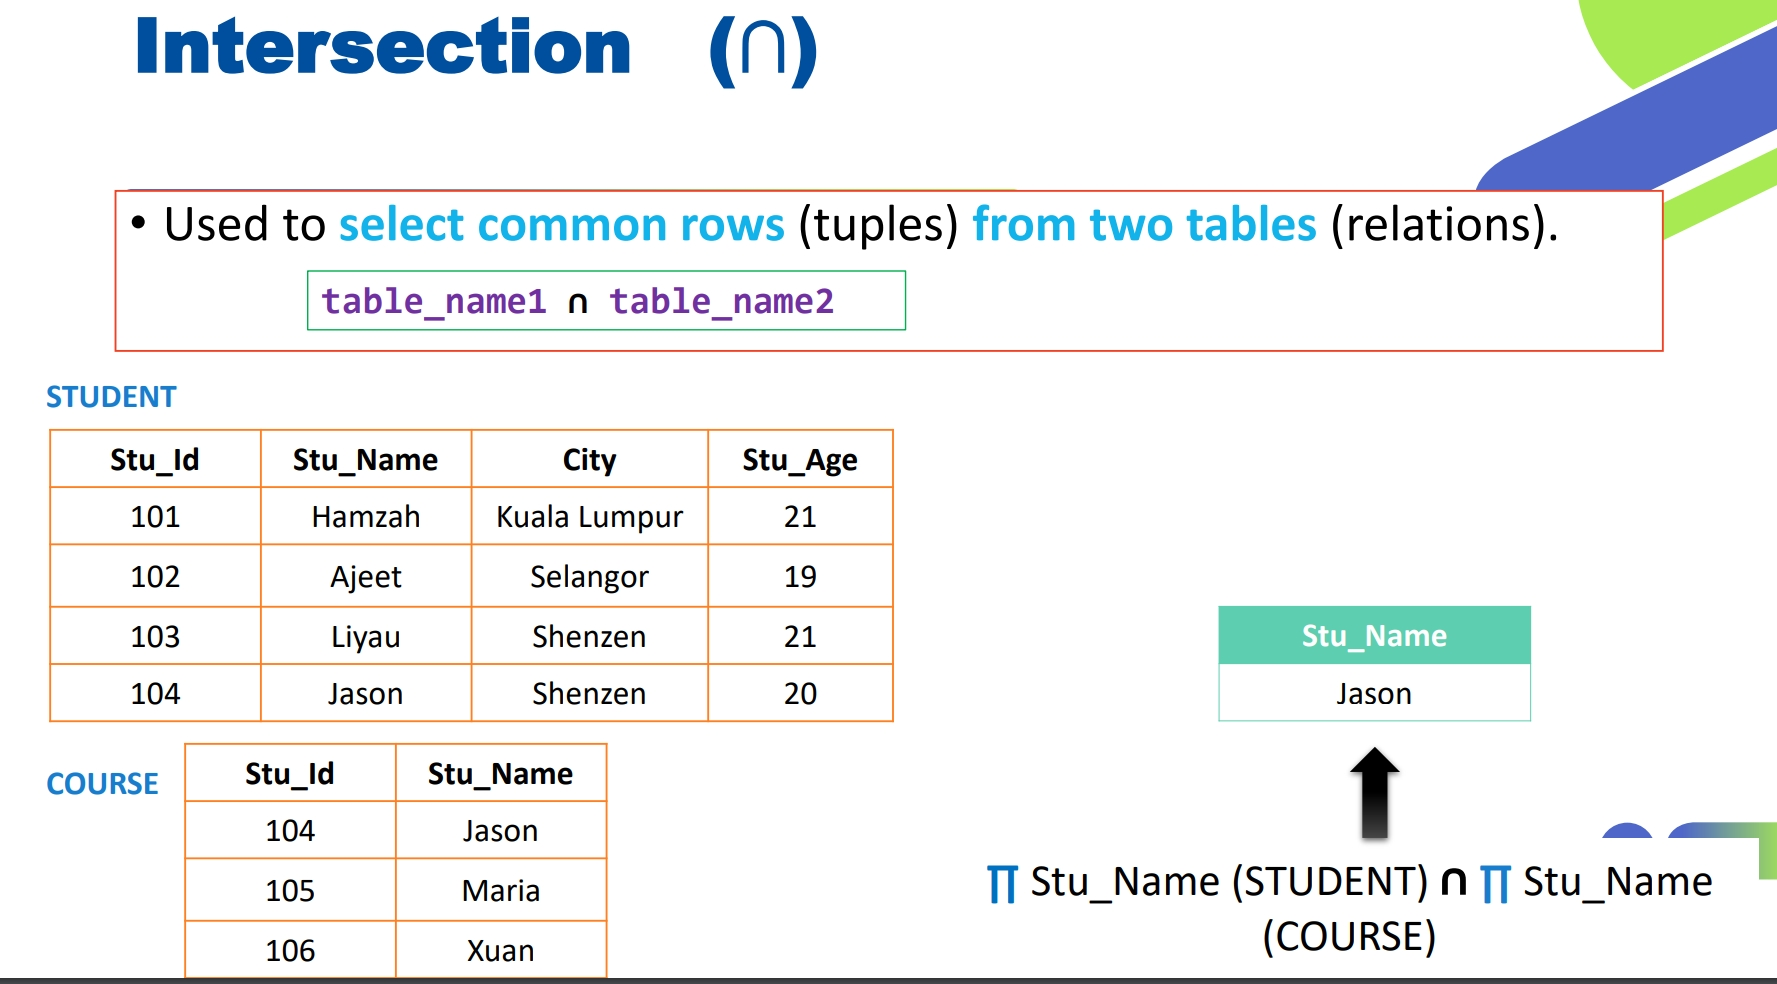
\includegraphics[width=0.9\textwidth]{chapter1a_11.png}
    \end{figure}
    \begin{figure}[H]
        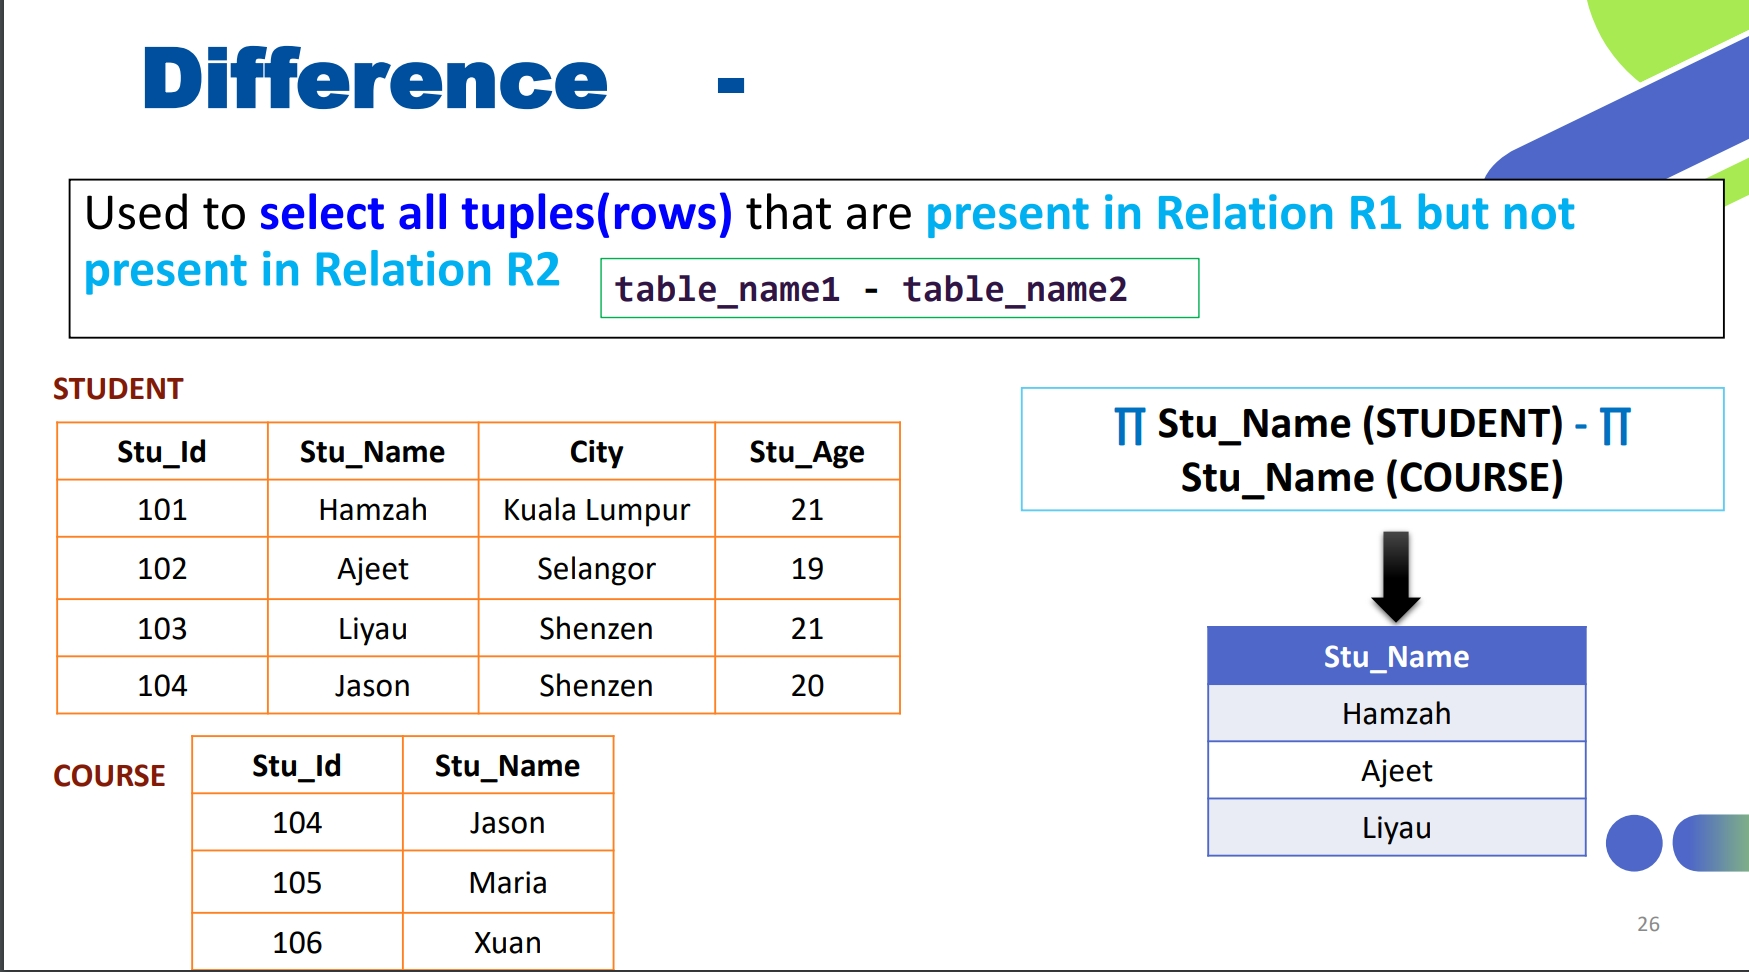
\includegraphics[width=0.9\textwidth]{chapter1a_12.png}
        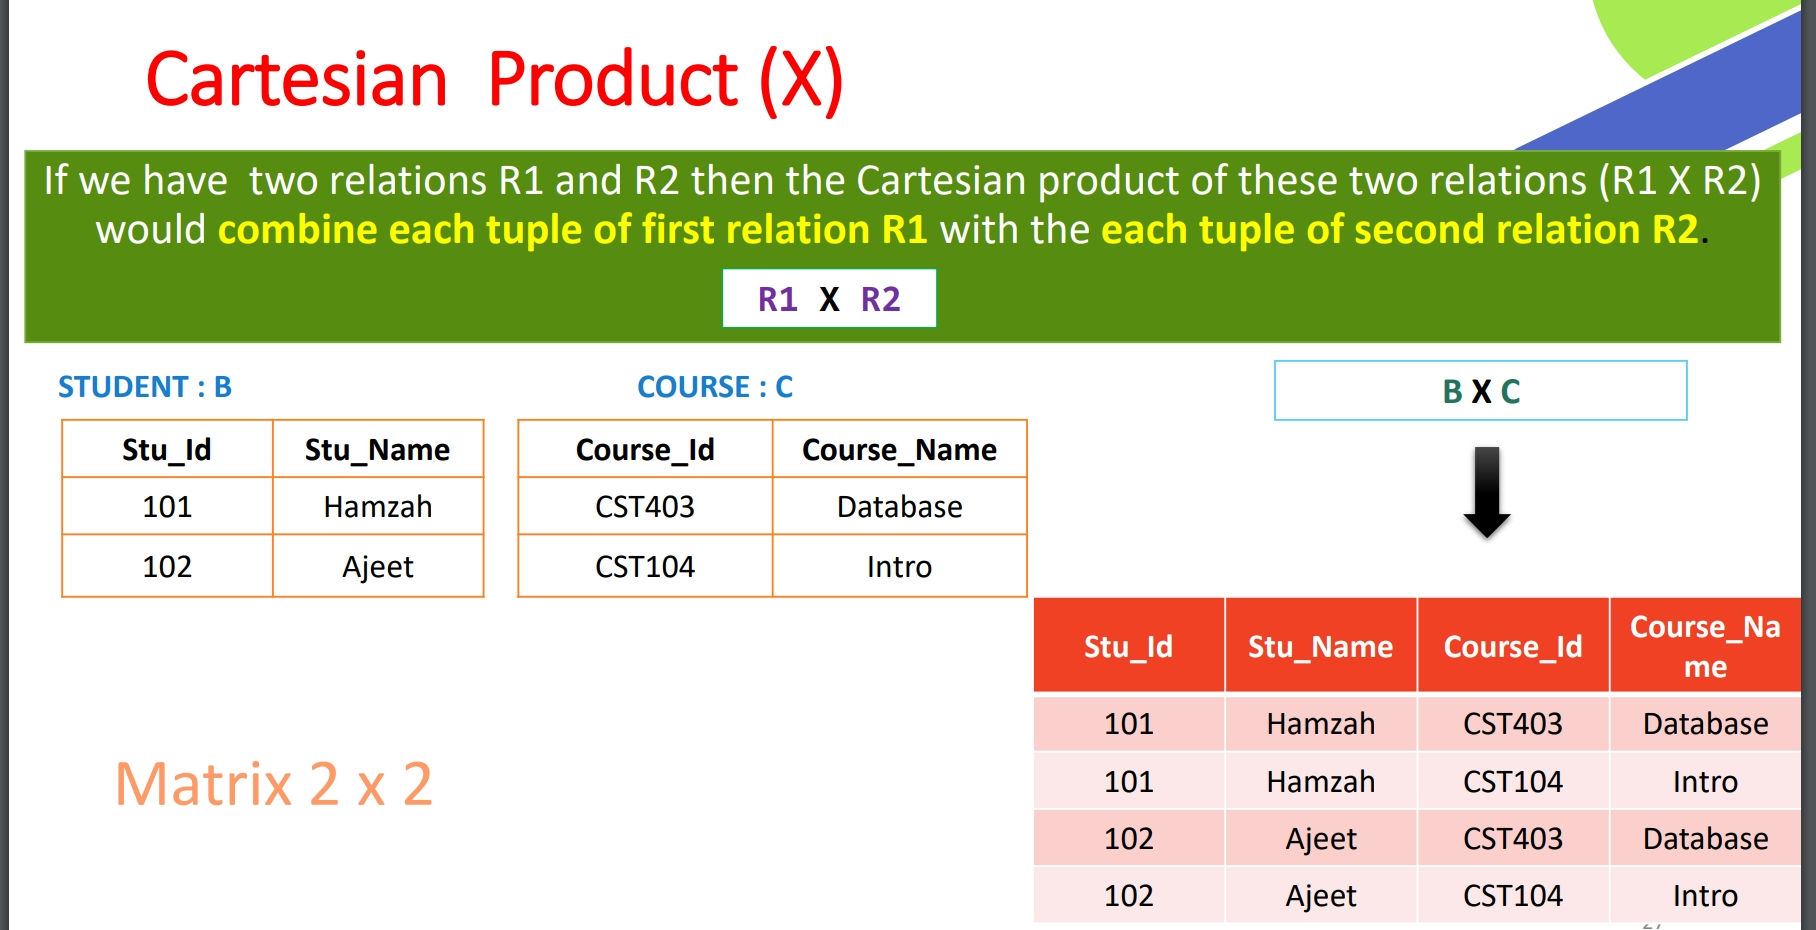
\includegraphics[width=0.9\textwidth]{chapter1a_13.png}
        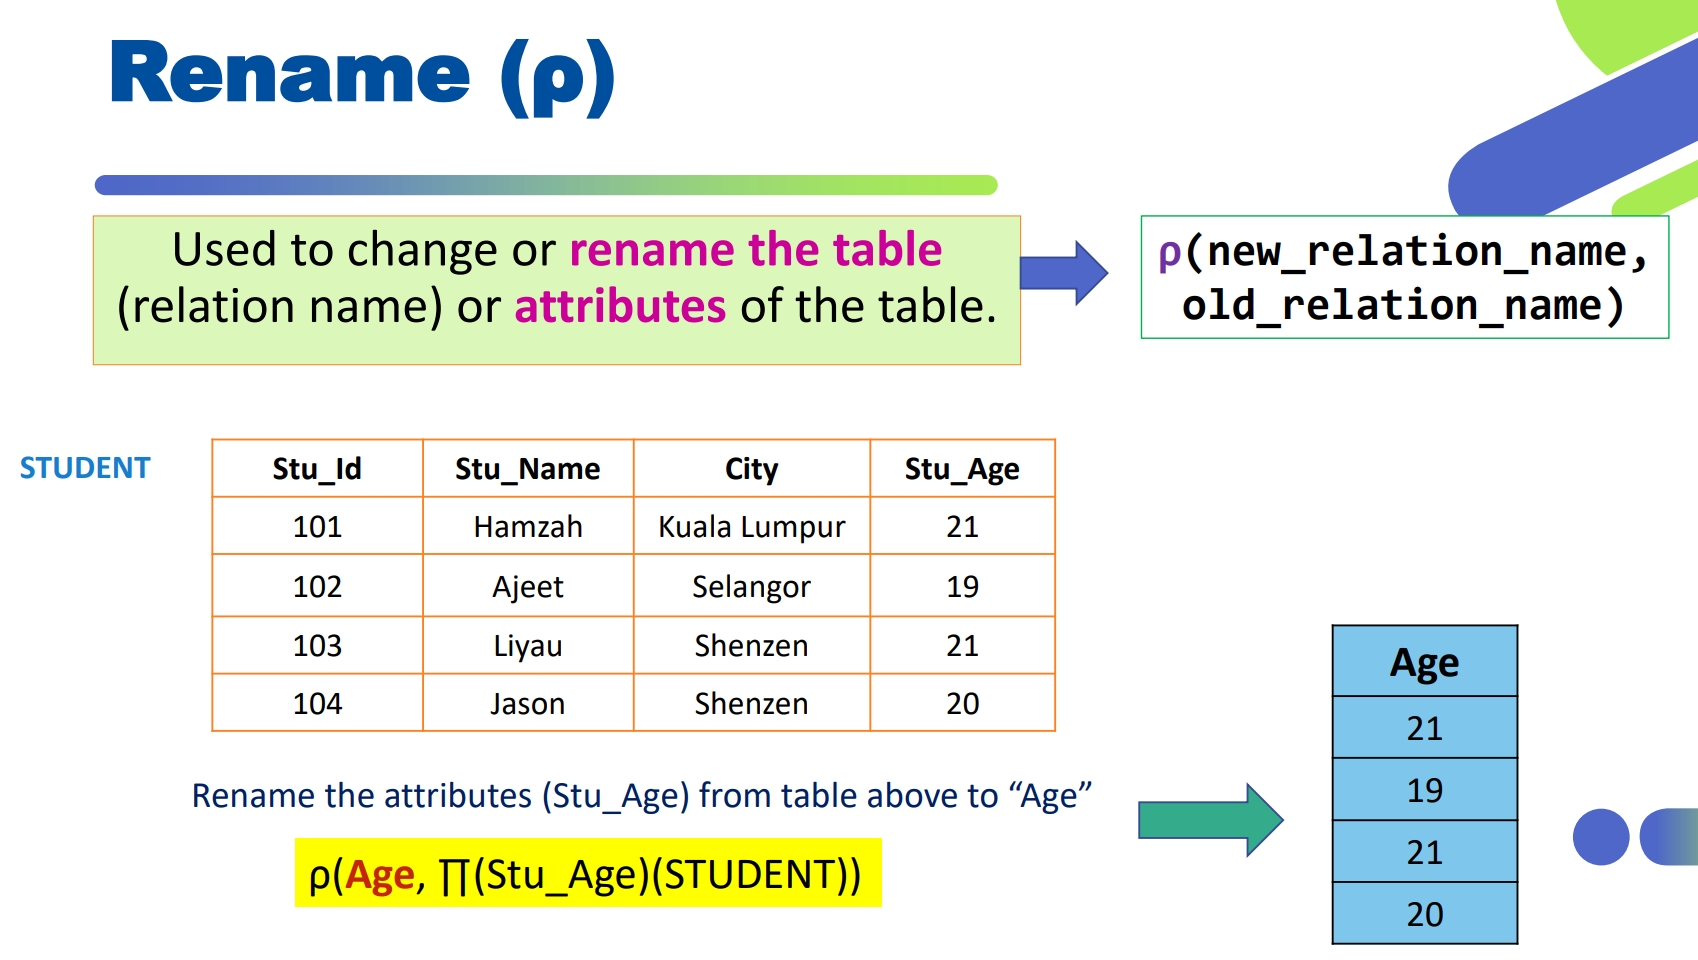
\includegraphics[width=0.9\textwidth]{chapter1a_14.png}
    \end{figure}
    \newpage
\section{2B: Entity Relationship Diagram}
\fancyhead[R]{October 10, 2024}
    \subsection{Entities}
        \begin{itemize}
            \item Person,place,objects,event or concept about which data is to be maintained.
            \item \textcolor{orange}{Box}
        \end{itemize}
    \subsection{Attributes}
        \begin{itemize}
            \item Properties or characteristic of an entity.
            \item Types
            \begin{itemize}
                \item Composite attributes
                \item Multi-valued attributes
                \item Derived attributes
            \end{itemize}
            \item \textcolor{orange}{Oval}
        \end{itemize}
    \subsection{Relationships}
    \begin{itemize}
        \item Verb phrase(belongs to)
        \item Association between the instances of one or more entities.
        \begin{itemize}
            \item One to one (1:1)
            \item One to many (1:M)
            \item Many to many (M:M)
        \end{itemize}
        \item \textcolor{orange}{Diamond box}
    \end{itemize}
    \begin{figure}[H]
        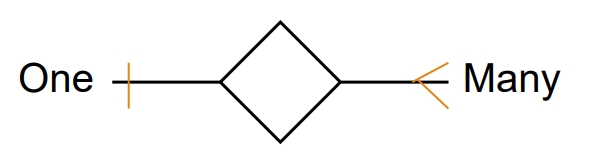
\includegraphics[width=0.3\textwidth]{chapter1a_15.png}
    \end{figure}

\newpage
\section{2C: Enhanced Entity Relationship Model(EERDM)}
\fancyhead[R]{October 3, 2024}

    \subsection{Chen Model vs Crow's Foot Model}
    \begin{figure}[H]
        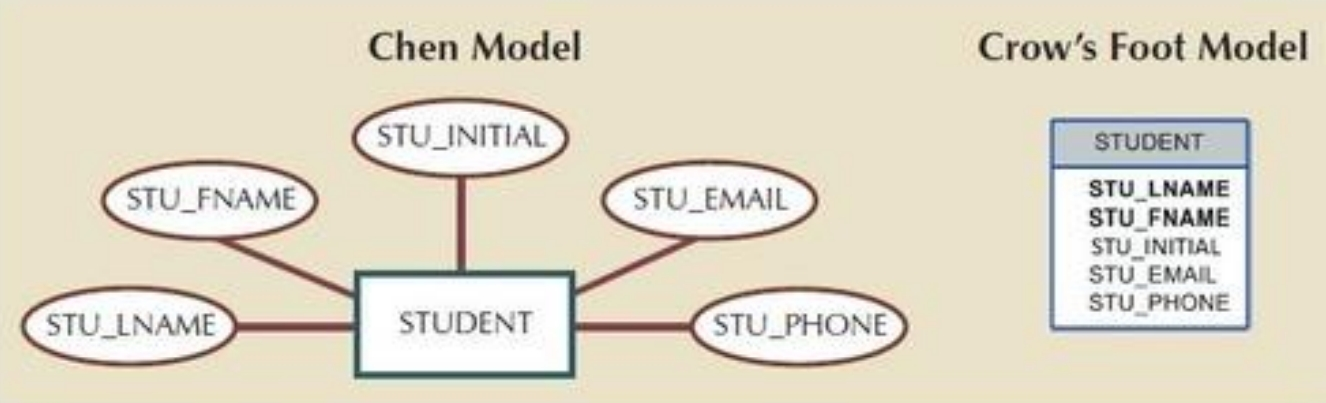
\includegraphics[width=\textwidth]{chapter2c_8.png}
    \end{figure}

    \subsection{Subclasses \& Superclasses}
        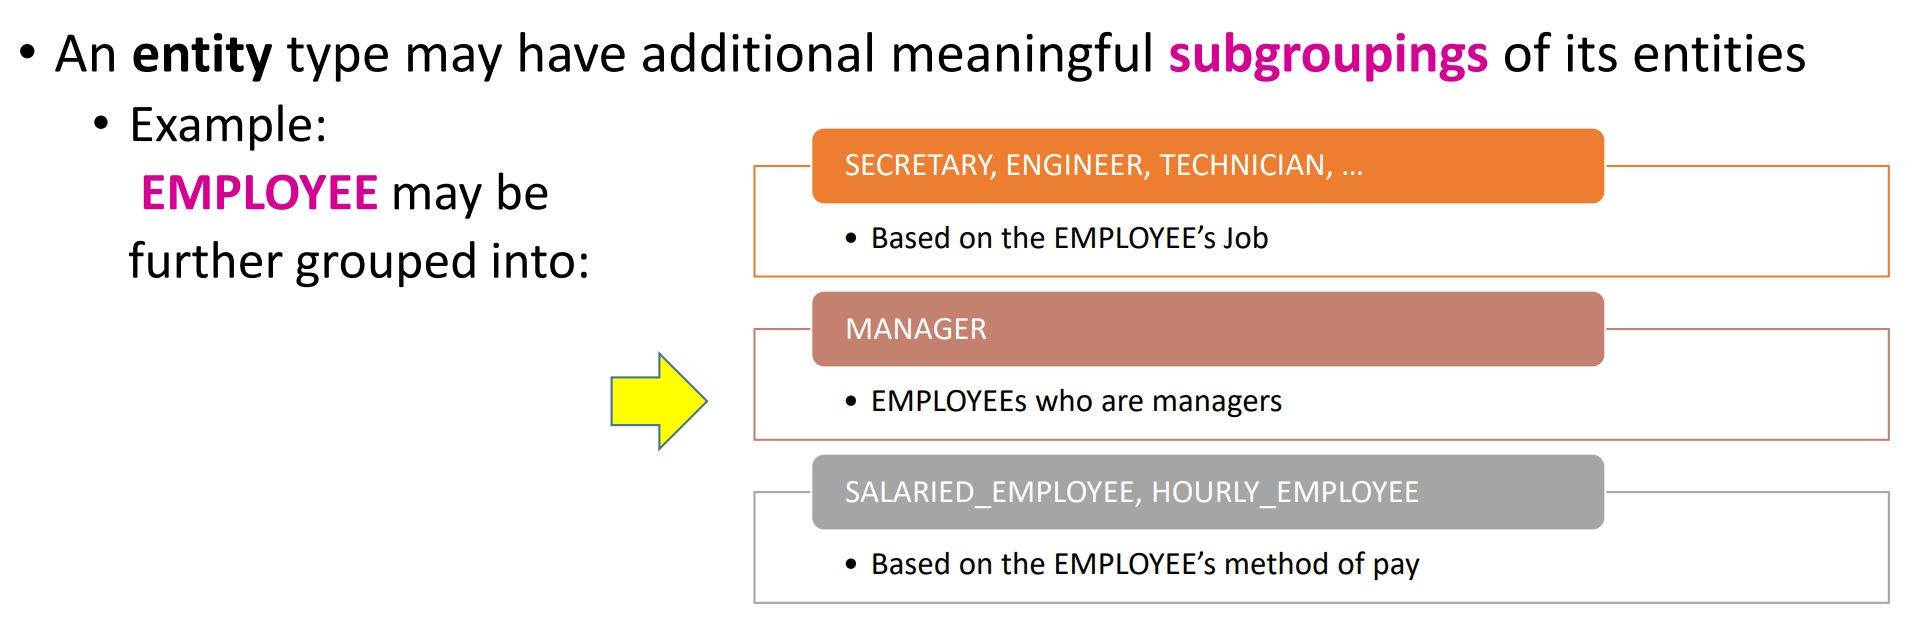
\includegraphics[width=\textwidth]{chapter2c_1.png}
        EER diagrams extend ER diagrams to represent these additional
        subgroupings, called subclasses or subtypes
        \begin{itemize}
            \item Each is called a \textbf{subclass} of EMPLOYEE
            \item EMPLOYEE is the \textbf{superclass} for each of these subclasses
            \item These are called superclass/subclass relationships:
            \begin{itemize}
                \item EMPLOYEE/SECRETARY
                \item EMPLOYEE/TECHNICIAN
                \item EMPLOYEE/MANAGER
            \end{itemize}
            \item These are also called \textcolor{red}{IS A} relationships
            \begin{itemize}
                \item SECRETARY IS-A EMPLOYEE, TECHNICIAN IS-A EMPLOYEE, ….
            \end{itemize}
        \end{itemize}

    \subsection{Generalization \& Specialization}
       \subsubsection{Generalize}
       \begin{itemize}
        \item A bottom-up strategy called generalization \textcolor{light-blue}{combines two lower level entities
        to create a higher level entity}.
        \item  Called a \textcolor{purple}{bottom up} conceptual synthesis process.
       \end{itemize}

       \subsubsection{Specialization}
       \begin{itemize}
        \item start with an entity type and then \textcolor{orange}{define subclasses of the entity} type by
        successive specialization.
        \item  called a \textcolor{brown}{top down} conceptual refinement process.
       \end{itemize}

       \subsubsection{Difference between Generalization \& Specialization}
       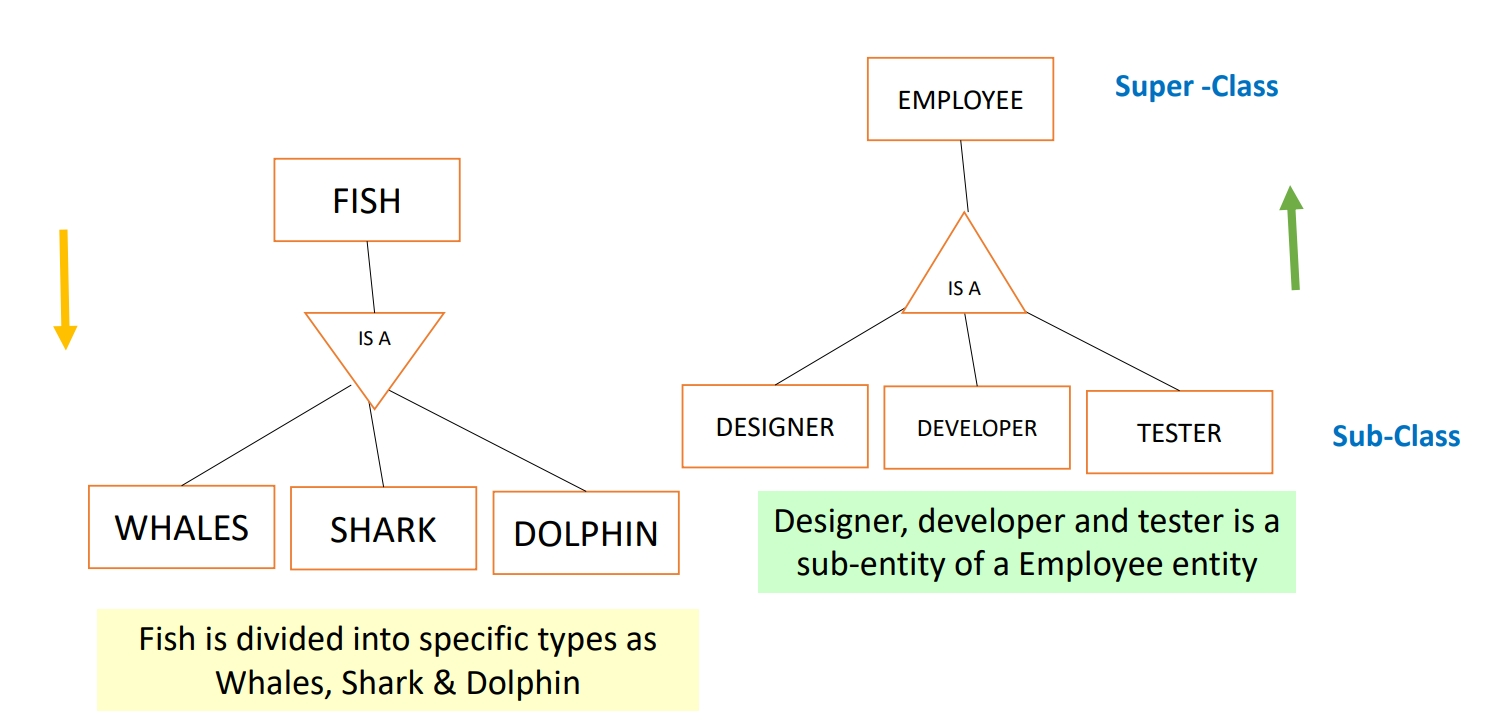
\includegraphics[width=\textwidth]{chapter2c_2.png}
        %\vspace{0.5cm} % Optional: Add some vertical space between images
       \textbf{Example:} % Text above the second image
       \begin{figure}[H]
        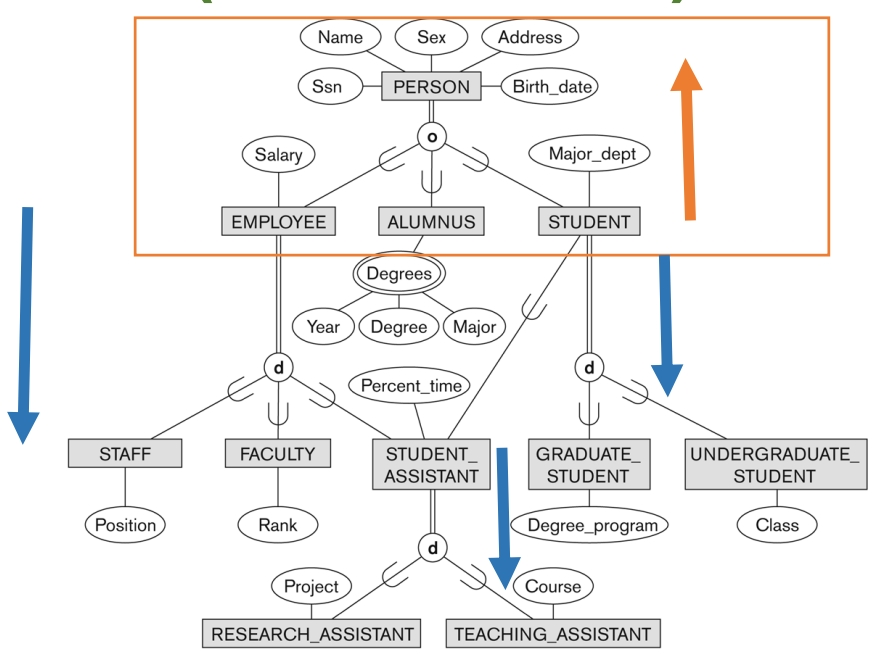
\includegraphics[width=0.8\textwidth]{chapter2c_3.png}
       \end{figure}

       \vspace{3cm}

       \textbf{Entity Before Generalization} % Text above the second image
       \begin{figure}[H]
        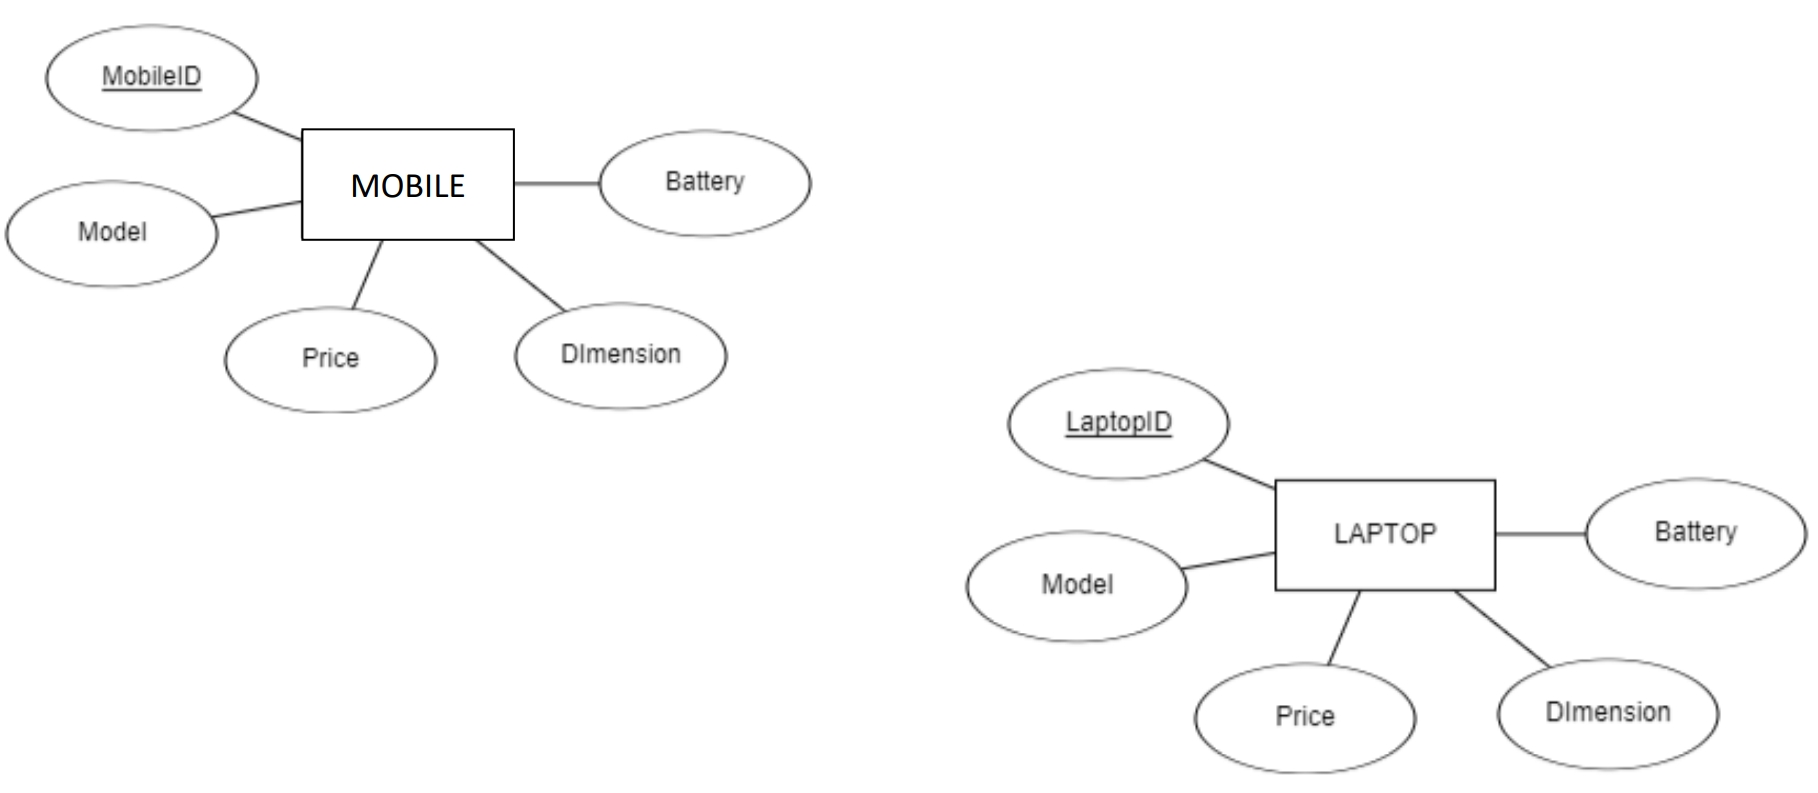
\includegraphics[width=\textwidth]{chapter2c_4.png}
       \end{figure}

       \textbf{Entity After Generalization} % Text above the second image
       \begin{figure}[H]
        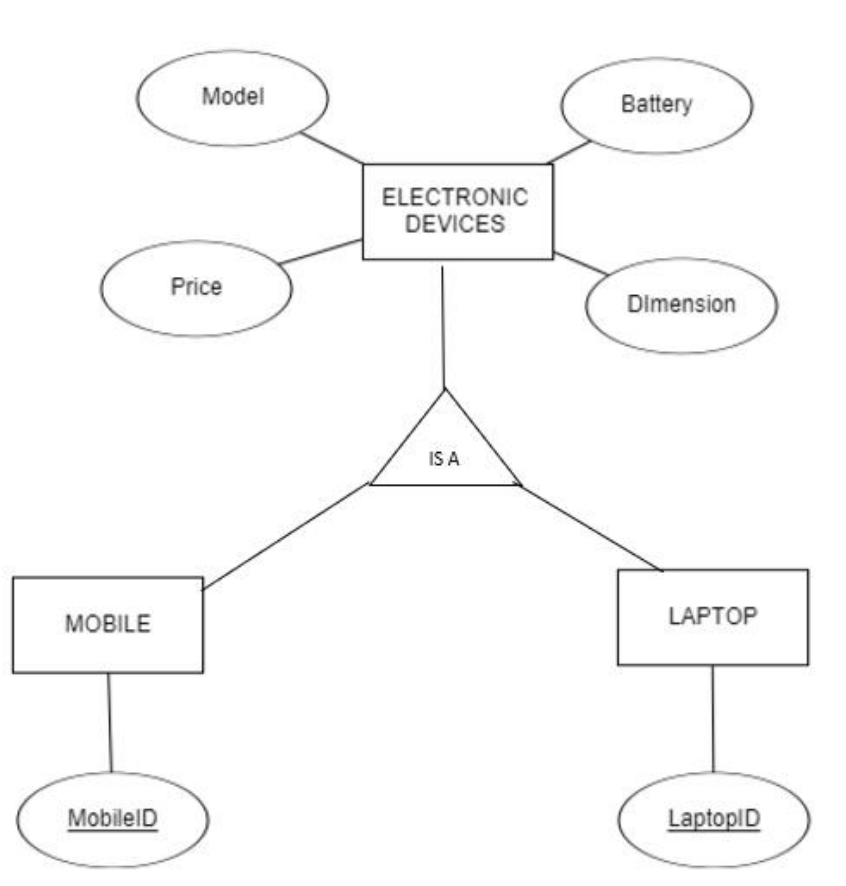
\includegraphics[width=0.8\textwidth]{chapter2c_5.png}
       \end{figure}

       \vspace{2cm}
       \textbf{Entity Before Specialization} % Text above the second image
       \begin{figure}[H]
        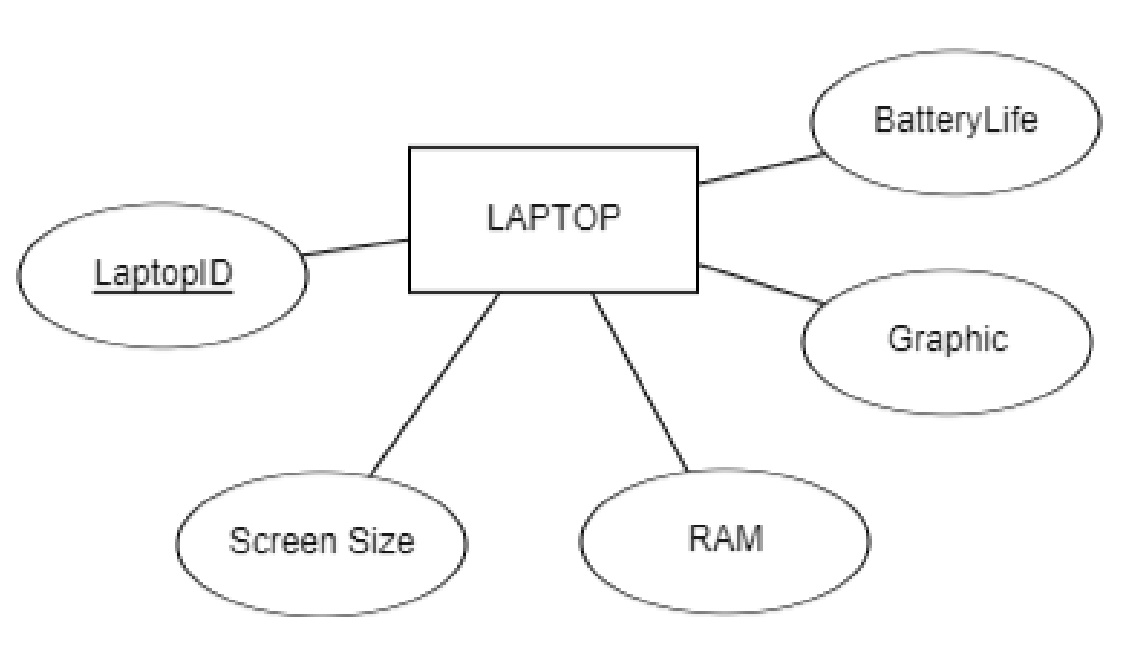
\includegraphics[width=0.8\textwidth]{chapter2c_6.png}
       \end{figure}

       \textbf{Entity AFTER Specialization} % Text above the second image
       \begin{figure}[H]
        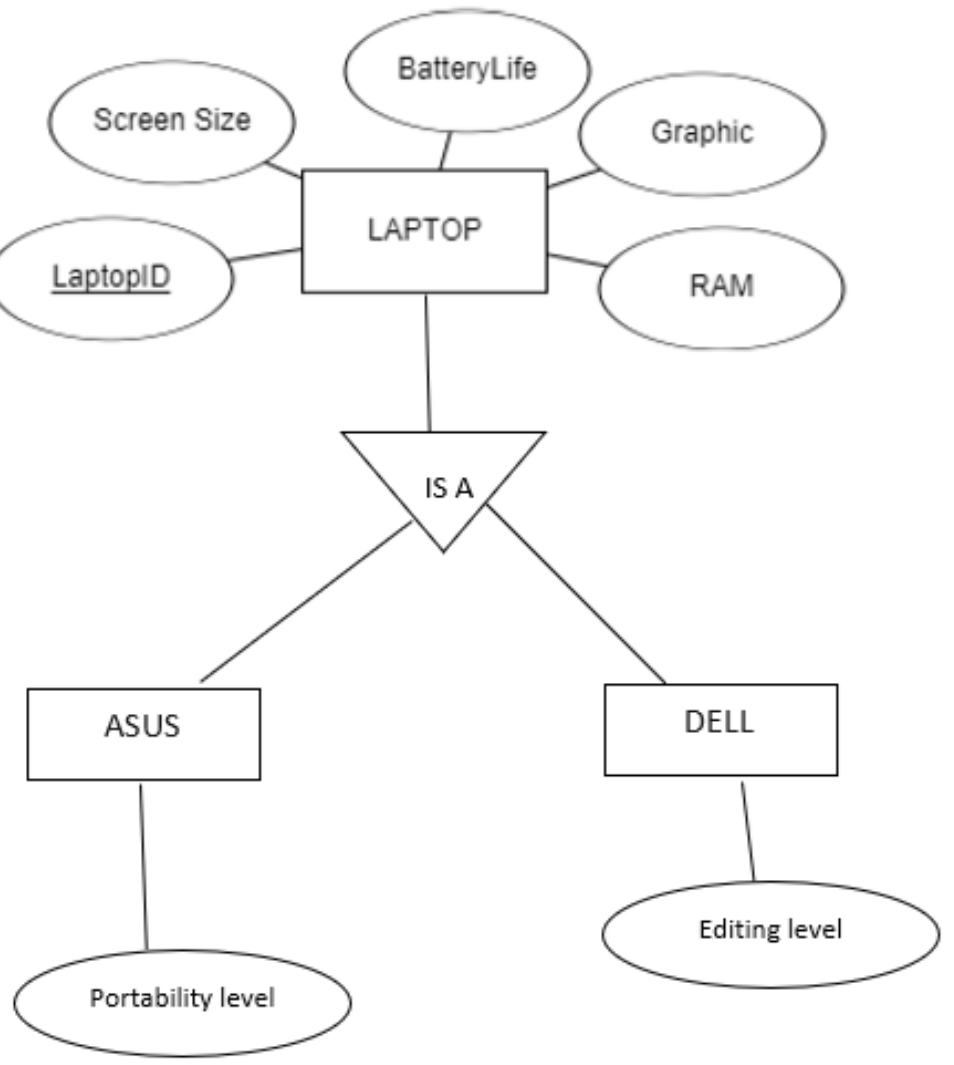
\includegraphics[width=0.8\textwidth]{chapter2c_7.png}
       \end{figure}
    \newpage
    \fancyhead[R]{October 10, 2024}
    \subsection{ERD $\rightarrow$ Relational Schema}
       \begin{figure}[H]
        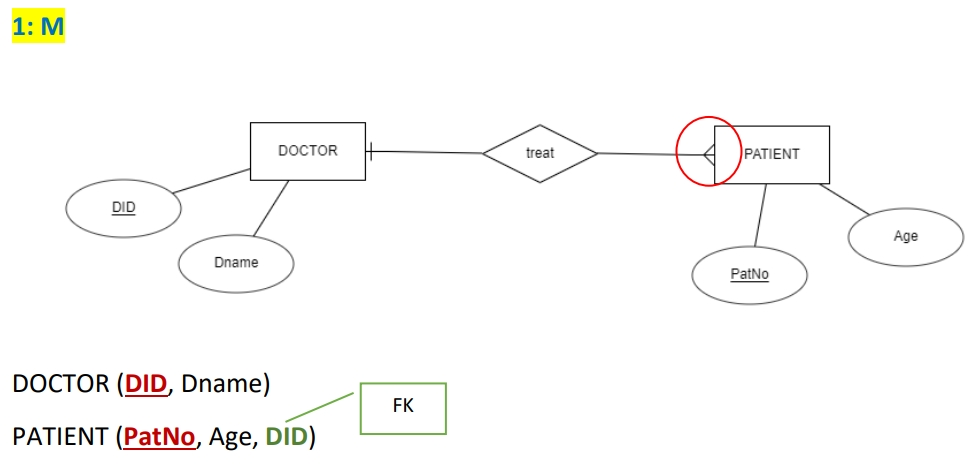
\includegraphics[width=0.8\textwidth]{chapter2c_9.png}
        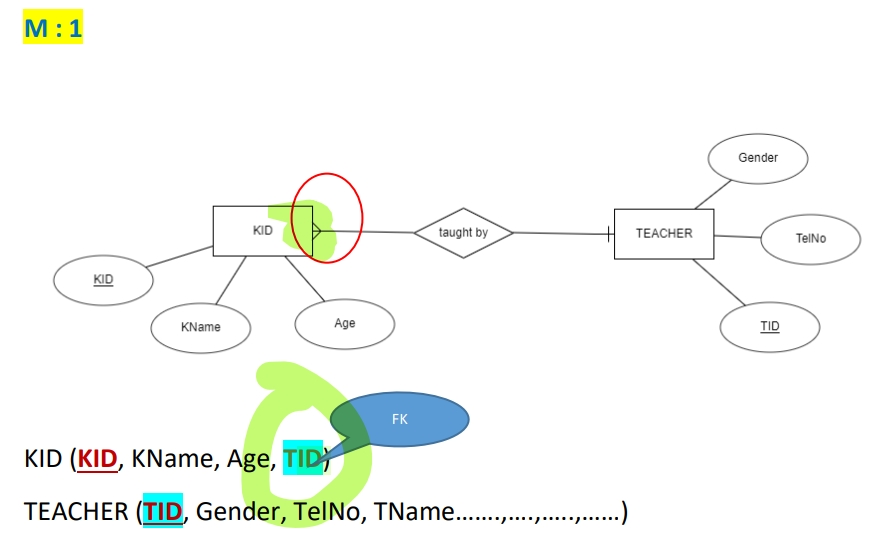
\includegraphics[width=0.8\textwidth]{chapter2c_10.png}
        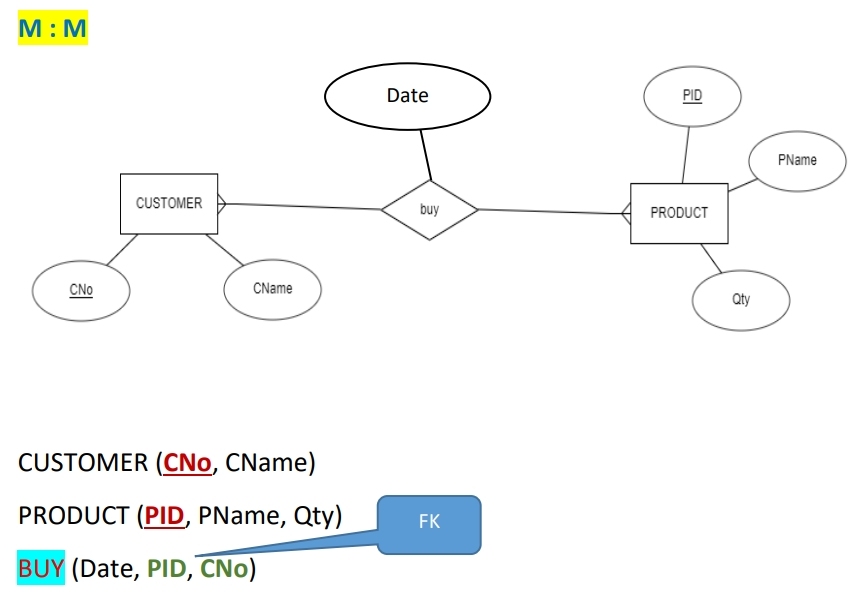
\includegraphics[width=0.8\textwidth]{chapter2c_11.png}
       \end{figure}
       \begin{figure}[H]  
        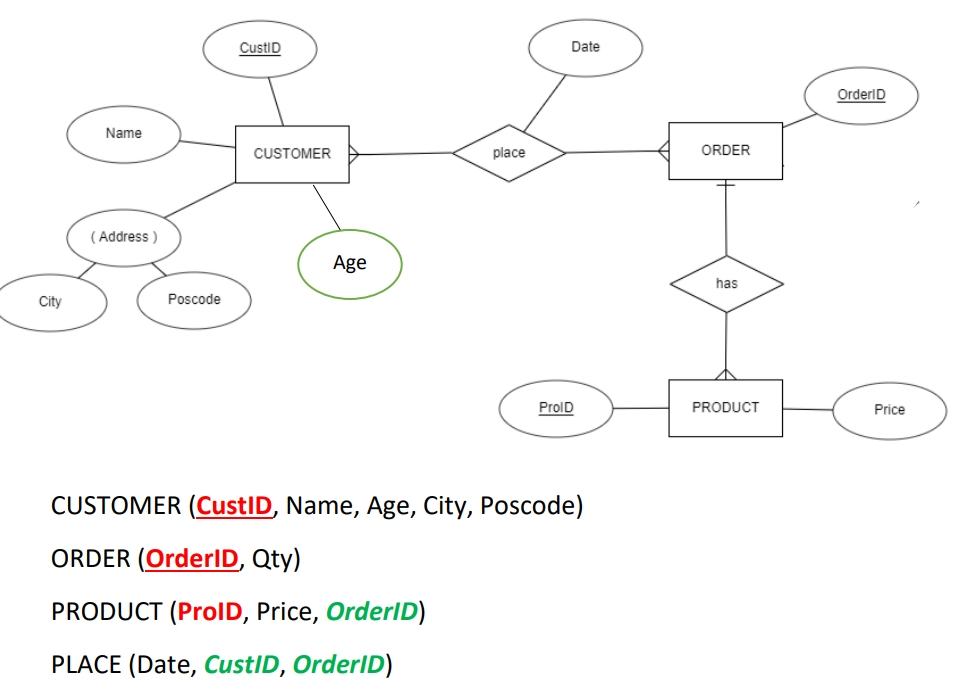
\includegraphics[width=0.8\textwidth]{chapter2c_12.png}
        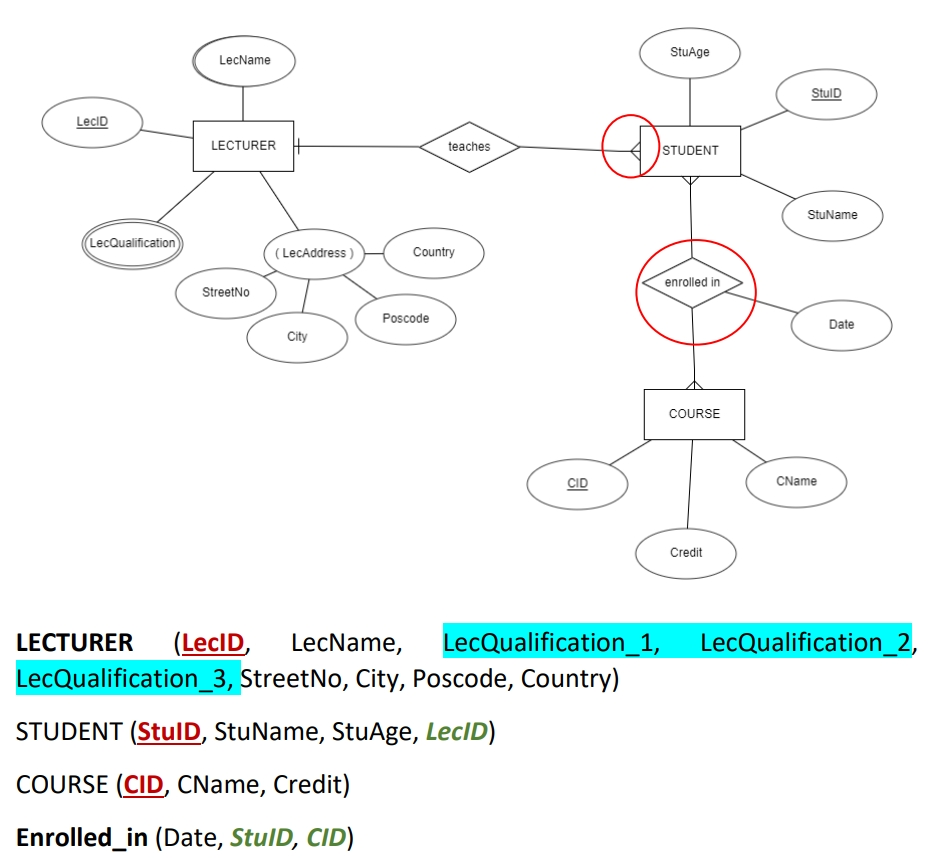
\includegraphics[width=0.8\textwidth]{chapter2c_13.png}
       \end{figure}

    \vspace{3cm}
    \subsection{Enhanced ERD $\rightarrow$ Relational Schema}
    \begin{figure}[H]
        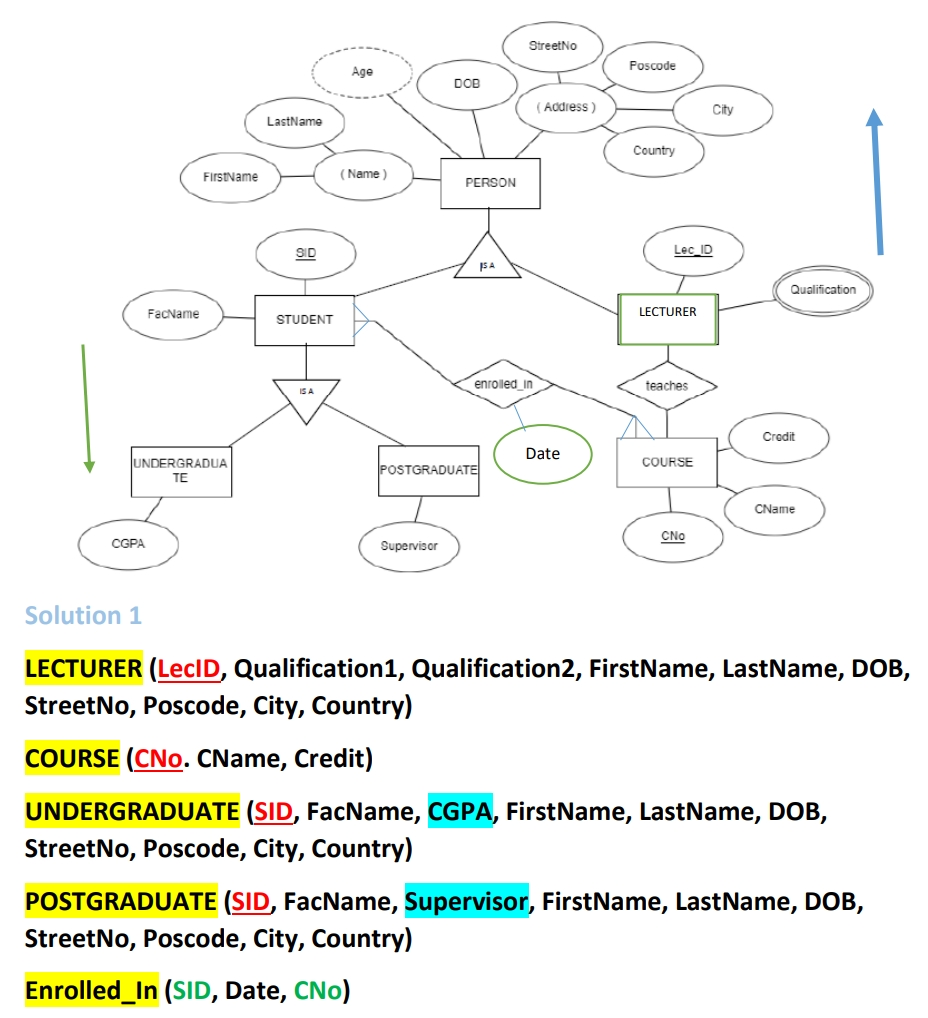
\includegraphics[width=0.8\textwidth]{chapter2c_14.png}
    \end{figure}

\newpage
\section{3A: Basic SQL}
\fancyhead[R]{October 10, 2024}
    \subsection{Structured Query Language}
    Considered one of the major reasons for the commercial success
    of relational databases.\\
    Others sql statements\\
    END
    

\end{document}
